% ============================================================================
% HOMEWORK ASSIGNMENT DOCUMENT
% ============================================================================

\documentclass[12pt]{article}

% ============================================================================
% PACKAGE IMPORTS
% ============================================================================
\usepackage{amsmath}
\usepackage{amssymb}
\usepackage{graphicx}
\usepackage{tikz}
\usepackage[margin=1in]{geometry}
\usepackage{setspace}
\usepackage{xcolor}
\usepackage{enumitem}
\usepackage{tcolorbox}
\usepackage{fancyhdr}
\usepackage{lastpage}
\usepackage{listings}
\lstset{
  basicstyle=\ttfamily\small,
  breaklines=true,
  breakatwhitespace=true,
  columns=fullflexible,
  keepspaces=true,
  frame=single,
  literate={–}{-}1 {—}{-}1 {…}{...}1 {’}{'}1 {“}{''}1 {”}{''}1
}

% ============================================================================
% CUSTOM TCOLORBOX STYLES
% ============================================================================
\newtcolorbox{hintbox}{
  colback=black!5,
  colframe=black,
  fonttitle=\bfseries,
  title=Hint,
  sharp corners,
  colbacktitle=black!15,
  coltitle=black
}

\newtcolorbox{stepbox}{
  colback=blue!5,
  colframe=blue!70!black,
  fonttitle=\bfseries,
  title=Step,
  sharp corners,
  colbacktitle=blue!15,
  coltitle=black
}

\newtcolorbox{codebox}{
  colback=green!5,
  colframe=green!70!black,
  fonttitle=\bfseries,
  title=MATLAB Implementation,
  sharp corners,
  colbacktitle=green!15,
  coltitle=black
}

\newtcolorbox{resultsbox}{
  colback=yellow!5,
  colframe=orange!70!black,
  fonttitle=\bfseries,
  title=Results,
  sharp corners,
  colbacktitle=orange!15,
  coltitle=black
}

% ============================================================================
% HEADER AND FOOTER SETUP
% ============================================================================
\pagestyle{fancy}
\setlength{\headheight}{14.5pt}
\fancyhf{}
\fancyhead[L]{Page \thepage\ of \pageref{LastPage}}
\fancyhead[C]{EMCH 721}
\fancyhead[R]{J.C. Vaught}
\renewcommand{\headrulewidth}{0pt}

% ============================================================================
% TIKZ LIBRARIES
% ============================================================================
\usetikzlibrary{shapes.geometric, arrows.meta, positioning, decorations.pathmorphing, patterns, calc}

% ============================================================================
% CUSTOM QUESTION COMMAND
% ============================================================================
\newcommand{\question}[1]{%
  \clearpage
  \vspace{0.5cm}
  {\noindent\normalsize \textbf{#1}}%
  \vspace{0.2cm}
  \hrule
  \vspace{0.1cm}
  \hrule
  \vspace{0.3cm}
}

\newcommand{\solutionframework}{%
\subsection*{Solution Outline}
\begin{stepbox}
\textbf{Planned Steps}\\[0.5em]
Outline your step-by-step approach here.
\end{stepbox}
\subsection*{MATLAB Implementation}
\begin{codebox}
Add MATLAB code or pseudocode here.
\end{codebox}
\subsection*{Results Summary}
\begin{resultsbox}
Summarize key intermediate and final results here.
\end{resultsbox}
}

% ============================================================================
% DOCUMENT INFORMATION
% ============================================================================
\title{EMCH 721: Homework 02}
\author{Instructor: Dr. Victor Giurgiutiu\\Student: J.C. Vaught}
\date{}

% ============================================================================
% BEGIN DOCUMENT
% ============================================================================
\begin{document}

\maketitle
\setlength{\parindent}{0pt}
\setstretch{1.1}

% List formatting defaults
\setlist[enumerate,1]{label=\arabic*.}
\setlist[enumerate,2]{label=\alph*.}

% ============================================================================
% TABLE OF CONTENTS
% ============================================================================
\begin{center}
\begin{tcolorbox}[colback=white, colframe=gray!50!black, colbacktitle=gray!20!white,
                  coltitle=black, sharp corners, boxrule=1pt,
                  title=\Large\bfseries Table of Contents]
\begin{tabular}{p{0.91\textwidth}r}
\textbf{A.1 Theoretical Analysis of SISO TF vs SS} \dotfill & \textbf{\pageref{quest:A1}} \\
\textbf{A.2 Numerical Work} \dotfill & \textbf{\pageref{quest:A2}} \\
\textbf{B.1 Time-Response Aeroelastic Model} \dotfill & \textbf{\pageref{quest:B1}} \\
\textbf{B.2 Setup for Time Response Flutter Calculations} \dotfill & \textbf{\pageref{quest:B2}} \\
\textbf{B.3 GVT Time Response} \dotfill & \textbf{\pageref{quest:B3}} \\
\textbf{B.4 Flutter Time Response} \dotfill & \textbf{\pageref{quest:B4}} \\
\textbf{B.5 Adjusted Flutter Speed} \dotfill & \textbf{\pageref{quest:B5}} \\
\textbf{C.1 Analysis} \dotfill & \textbf{\pageref{quest:C1}} \\
\textbf{C.2 Numerical Calculation} \dotfill & \textbf{\pageref{quest:C2}} \\
\textbf{D.1 Theoretical Model for Feedback Control of Flutter} \dotfill & \textbf{\pageref{quest:D1}} \\
\textbf{D.2 Setup for Feedback Control of Flutter} \dotfill & \textbf{\pageref{quest:D2}} \\
\textbf{D.3 Feedback Control of Flutter} \dotfill & \textbf{\pageref{quest:D3}} \\
\textbf{E.1 Theoretical Model for Flutter Control Through Aileron Feedback} \dotfill & \textbf{\pageref{quest:E1}} \\
\textbf{E.2 Setup for Flutter Control Through Aileron Feedback} \dotfill & \textbf{\pageref{quest:E2}} \\
\textbf{E.3 Flutter Control Through Aileron Feedback} \dotfill & \textbf{\pageref{quest:E3}} \\
\textbf{F.1 Negative Damping Suppression in GVT Conditions} \dotfill & \textbf{\pageref{quest:F1}} \\
\textbf{Appendix A: MATLAB Source Listings} \dotfill & \textbf{\pageref{appendix:matlab}} \\
\end{tabular}
\vspace{0.2cm}
\end{tcolorbox}
\end{center}

\clearpage

% ============================================================================
% PROBLEM CONTEXT
% ============================================================================
\section*{Problem Context}

Consider an airfoil in wind tunnel testing with airspeed $U$ (Figure~\ref{fig:airfoil-overview}). The airfoil is supported by springs and dampers at point $P$. The center of mass is at $C$. The distance from $P$ to $C$ is the static offset $x_{CP}$. The aerodynamic lift $L$ acts at point $Q$. The distance from $P$ to $Q$ is the aerodynamic offset $x_{QP}$. The airfoil undergoes oscillatory motion with plunge displacement $h(t)$ and pitch displacement $\theta(t)$. The positive plunge direction is downward. The positive pitch direction is ``nose up'' (clockwise).

\begin{figure}[htbp]
  \centering
  \providecolor{UofSCGarnet}{RGB}{115, 0, 10}
\providecolor{UofSCBlack}{RGB}{0, 0, 0}
\providecolor{UofSCWhite}{RGB}{255, 255, 255}
\providecolor{UofSC90Black}{RGB}{54, 54, 54}
\providecolor{UofSC70Black}{RGB}{92, 92, 92}
\providecolor{UofSC50Black}{RGB}{162, 162, 162}
\providecolor{UofSC30Black}{RGB}{199, 199, 199}
\providecolor{UofSC10Black}{RGB}{235, 235, 235}
\providecolor{UofSCWarmGrey}{RGB}{103, 97, 86}
\providecolor{UofSCSandstorm}{RGB}{255, 242, 227}
\providecolor{UofSCRose}{RGB}{204, 46, 64}
\providecolor{UofSCAtlantic}{RGB}{70, 106, 159}
\providecolor{UofSCCongaree}{RGB}{31, 65, 77}
\providecolor{UofSCHorseshoe}{RGB}{101, 120, 11}
\providecolor{UofSCGrass}{RGB}{206, 211, 24}
\providecolor{UofSCHoneycomb}{RGB}{164, 145, 55}
\providecolor{UofSCDarkGarnet}{RGB}{87, 0, 8}
\providecolor{UofSCAzalea}{RGB}{132, 66, 71}

\newcommand{\IsoViewDiagram}{%
    \begin{tikzpicture}[x={(0.866cm,-0.4cm)}, y={(0.6cm,0.5cm)}, z={(0cm,1cm)}, scale=1.3]

        \def\span{6}
        \def\chord{3}

        \fill[UofSCWarmGrey!60] (0, -1, -2) -- (0, \chord+1, -2) -- (0, \chord+1, 2) -- (0, -1, 2) -- cycle;
        \draw[thick] (0, -1, -2) -- (0, \chord+1, -2) -- (0, \chord+1, 2) -- (0, -1, 2) -- cycle;

        \newcommand{\drawAirfoilIso}[1]{%
            plot [smooth cycle, tension=0.6] coordinates {
                (##1, 0, 0)
                (##1, 0.2*\chord, 0.1*\chord)
                (##1, 0.6*\chord, 0.08*\chord)
                (##1, \chord, 0)
                (##1, 0.6*\chord, -0.05*\chord)
                (##1, 0.2*\chord, -0.08*\chord)
            }
        }

        \draw[thick, UofSCBlack] (0, \chord, 0) -- (\span, \chord, 0);
        \draw[thick, UofSCBlack] (0, 0, 0) -- (\span, 0, 0);
        \draw[thick, fill=UofSC10Black] \drawAirfoilIso{\span};
        \draw[dashed, thick] \drawAirfoilIso{0};

        \coordinate (RootQ) at (0, 0.2*\chord, 0);
        \coordinate (TipQ) at (\span, 0.2*\chord, 0);
        \draw[densely dotted, UofSCAtlantic, thick] (RootQ) -- (TipQ);
        \node[right, font=\footnotesize, UofSCAtlantic] at (\span+0.3, 0.2*\chord, 0) {$Q_{\text{axis}}$};
        \fill[UofSCAtlantic] (TipQ) circle (1pt);

        \coordinate (RootC) at (0, 0.4*\chord, 0);
        \coordinate (TipC) at (\span, 0.4*\chord, 0);
        \draw[densely dotted, UofSCBlack, thick] (RootC) -- (TipC);
        \node[right, font=\footnotesize, UofSCBlack] at (\span+0.3, 0.4*\chord, 0) {$C_{\text{axis}}$};
        \fill[UofSCBlack] (TipC) circle (1pt);

        \coordinate (RootP) at (0, 0.6*\chord, 0);
        \coordinate (TipP) at (\span, 0.6*\chord, 0);
        \draw[dashed, UofSCGarnet, thick] (RootP) -- (TipP);
        \node[right, font=\footnotesize, UofSCGarnet] at (\span+0.3, 0.6*\chord, 0) {$P_{\text{axis}}$};
        \fill[UofSCGarnet] (TipP) circle (1pt);

        \fill[UofSCAtlantic!40, opacity=0.9]
            plot [smooth, tension=0.6] coordinates {(0,0,0) (0, 0.2*\chord, 0.1*\chord) (0, 0.6*\chord, 0.08*\chord) (0,\chord,0)}
            --
            plot [smooth, tension=0.6] coordinates {(\span,\chord,0) (\span, 0.6*\chord, 0.08*\chord) (\span, 0.2*\chord, 0.1*\chord) (\span,0,0)}
            -- cycle;

        \draw[thick] (0,0,0) -- (\span,0,0);
        \draw[thick] (0,\chord,0) -- (\span,\chord,0);
        \draw[thick] \drawAirfoilIso{\span};

        \draw[->, thick, UofSCGarnet] (0, \chord, 0) -- (\span + 0.5, \chord, 0) node[right] {$z$ (Span)};

        \foreach \x in {1, 2, 3, 4, 5} {
            \draw[->, ultra thick, UofSCGarnet] (\x, -1.2, 0) -- (\x, -0.2, 0);
        }
        \node[right, UofSCGarnet] at (3, -2.0, 0) {$U$};

        \node[align=center] at (\span+0.5, \chord+0.5, 0.5) {Tip (Free)};
        \node[align=center] at (-0.5, \chord/2, 2.5) {Root (Fixed)};
    \end{tikzpicture}%
}

\providecolor{UofSCGarnet}{RGB}{115, 0, 10}
\providecolor{UofSCBlack}{RGB}{0, 0, 0}
\providecolor{UofSCAtlantic}{RGB}{70, 106, 159}
\providecolor{UofSCLightGray}{RGB}{200, 200, 200}

\newcommand{\CrossSectionDiagram}{%
    \begin{tikzpicture}[scale=1.5, >=Latex]
        \draw[thick, fill=UofSCLightGray] plot [smooth cycle, tension=0.6] coordinates {
            (0,0)
            (1.2, 0.6)
            (3.6, 0.48)
            (6,0)
            (3.6, -0.3)
            (1.2, -0.48)
        };

        \draw[dashed, UofSCBlack] (-0.2,0) -- (6.5,0) node[right] {Reference Chord Line};

        \coordinate (Q) at (1.2,0);
        \coordinate (C) at (2.4,0);
        \coordinate (P) at (3.6,0);

        \draw[<->, thick] ($(Q)+(0,1)$) -- ($(P)+(0,1)$) node[midway, fill=white] {$x_{QP}$};
        \draw[dashed] (P) -- ($(P)+(0,1.2)$);
        \draw[<->, thick] ($(P)+(0,0.75)$) -- ($(C)+(0,0.75)$) node[midway, fill=white] {$x_{CP}$};
        \draw[dashed] (C) -- ($(C)+(0,0.8)$);

        \fill[UofSCGarnet] (P) circle (2pt) node[below=7mm] {P};
        \fill[UofSCBlack] (C) circle (2pt) node[below=7mm] {C};
        \fill[UofSCAtlantic] (Q) circle (2pt) node[below=7mm] {Q};

        \draw[->, ultra thick, UofSCAtlantic] (-2, 0) -- (-0.5, 0) node[above] {$U$};

        \draw[->, ultra thick, UofSCAtlantic] (Q) -- ($(Q)+(0,1.5)$) node[right] {$L(U)$};

        \draw[->, ultra thick, UofSCGarnet] ($(Q)+(-2,-0.4)$) arc (270:90:0.4) node[midway, above left] {$\theta(z,t)$};
    \end{tikzpicture}%
}


\IsoViewDiagram

\vspace{1em}

\CrossSectionDiagram

  \caption{Overview of the plunging-pitching airfoil with reference points and offsets $x_{CP}$, $x_{QP}$.}
  \label{fig:airfoil-overview}
\end{figure}


\subsection*{Notes}
\begin{tcolorbox}[colback=white,colframe=black,colbacktitle=gray!20!white,
                  coltitle=black,sharp corners,boxrule=1pt,
                  title=Submission Notes]
\begin{itemize}[leftmargin=1.2em]
  \item Always display input data.
  \item Show work and relevant comments.
  \item Attach MATLAB codes to receive partial credit where applicable.
  \item Report numerical results to three significant digits (use four if the first digit is 1).
  \item Problems solved beyond the minimum requirements may receive bonus points.
  \item Challenge problems are optional and count toward extra credit.
\end{itemize}
\end{tcolorbox}

\subsection*{Input Data}
\begin{tcolorbox}[colback=white,colframe=black,colbacktitle=gray!20!white,
                  coltitle=black,sharp corners,boxrule=1pt,
                  title=Input Data Summary]
\begin{tabular}{@{}ll@{}}
\textbf{Parameter} & \textbf{Value} \\
Air density $\rho$ & $1.225~\mathrm{kg/m^3}$ \\
Chord $c$ & $0.4~\mathrm{m}$ \\
Mass $m$ & $2.8~\mathrm{kg}$ \\
Mass moment of inertia $I_0$ & $0.05~\mathrm{kg\cdot m^2}$ \\
Plunge frequency $f_h$ & $1.6~\mathrm{Hz}$ \\
Pitch frequency $f_\theta$ & $4.8~\mathrm{Hz}$ \\
Plunge damping ratio $\zeta_h$ & $2\%$ \\
Pitch damping ratio $\zeta_\theta$ & $3\%$ \\
Static offset $x_{CP}$ & $-10\%\,c$ \\
Aerodynamic offset $x_{QP}$ & $30\%\,c$ \\
\end{tabular}
\end{tcolorbox}

\subsection*{Notations}
\begin{tcolorbox}[colback=white,colframe=black,colbacktitle=gray!20!white,
                  coltitle=black,sharp corners,boxrule=1pt,
                  title=Notation Reference]
\begin{tabular}{@{}ll@{}}
\textbf{Symbol} & \textbf{Meaning} \\
EOM & Equation of motion \\
CL & Closed loop \\
FBD & Free body diagram \\
FB & Feedback \\
GVT & Ground vibration test \\
LHS & Left-hand side \\
LT & Laplace transform \\
MIMO & Multi-input multi-output \\
ODE & Ordinary differential equation \\
PDE & Partial differential equation \\
RHS & Right-hand side \\
SISO & Single-input single-output \\
SS & State space \\
TF & Transfer function \\
\end{tabular}
\end{tcolorbox}

% ============================================================================
% QUESTIONS
% ============================================================================

\question{A.1 Theoretical Analysis of SISO TF vs SS}\label{quest:A1}

Recall the one-degree-of-freedom damped forced vibration equation in standard form in terms of natural frequency $\omega_n$ and damping ratio $\zeta$. This ordinary differential equation (ODE) describes how a second-order dynamic system responds to a forcing function $f(t)$. The solution of this ODE is the system response $x(t)$.
\begin{enumerate}[label=(\alph*)]
  \item Express the second-order dynamic system as a transfer function (TF) representation in the Laplace domain $s$.
  \item Recast the second-order dynamic system into a first-order extended state-space (SS) system representation in the time domain $t$ using the vectors $z$, $u$, and $y$.
  \item Show the relationship between $z$, $u$, $y$ and $x$, $f$.
  \item Derive the state-space matrices $A$, $B$, $C$, and $D$.
\end{enumerate}

\subsection*{Solution for Part (a)}

\begin{stepbox}
\textbf{Step 1: Start from the physical equation of motion}\\[0.5em]
The single-degree-of-freedom aeroelastic mode behaves as a damped oscillator excited by an external force $f^\ast(t)$. Its governing ordinary differential equation is
\[
m\,\ddot{x}(t) + c\,\dot{x}(t) + k\,x(t) = f^\ast(t),
\]
where $m$ is the modal mass, $c$ the structural (or aerodynamic) damping, and $k$ the generalized stiffness.  Dividing through by $m$ exposes the dimensionless dynamics:
\[
\ddot{x}(t) + \frac{c}{m}\,\dot{x}(t) + \frac{k}{m}\,x(t) = \frac{1}{m}\,f^\ast(t).
\]
Introduce the natural frequency $\omega_n = \sqrt{\tfrac{k}{m}}$ and damping ratio $\zeta = \tfrac{c}{2\sqrt{km}}$ so that the excitation is written with a normalized input force $f(t)=\tfrac{k}{m}f^\ast(t)$,
\[
\ddot{x}(t) + 2\zeta\omega_n\,\dot{x}(t) + \omega_n^2\,x(t) = \omega_n^2\,f(t).
\]
This manipulation isolates the fundamental modal properties $(\omega_n,\zeta)$ that will carry directly into the transfer-function coefficients.
\end{stepbox}

\begin{stepbox}
\textbf{Step 2: Apply the Laplace transform term by term}\\[0.5em]
To convert the time-domain differential equation into an algebraic $s$-domain expression we use the Laplace transform definition $\mathcal{L}\{g(t)\} = \int_0^{\infty} g(t)\,e^{-st}\,\mathrm{d}t$ and its derivative identities
\[
\mathcal{L}\{\dot{g}(t)\} = sG(s) - g(0), \qquad
\mathcal{L}\{\ddot{g}(t)\} = s^2 G(s) - s g(0) - \dot{g}(0).
\]
For an aeroelastic response that is initially at rest we set $x(0)=0$ and $\dot{x}(0)=0$.  Taking the Laplace transform of each term in the normalized equation from Step~1 therefore yields
\[
\mathcal{L}\{\ddot{x}\} = s^2 X(s), \qquad
\mathcal{L}\{2\zeta\omega_n \dot{x}\} = 2\zeta\omega_n\, s X(s), \qquad
\mathcal{L}\{\omega_n^2 x\} = \omega_n^2 X(s),
\]
while the right-hand side becomes $\mathcal{L}\{\omega_n^2 f(t)\} = \omega_n^2 F(s)$.  Substituting these pieces back into the transformed equation gives the compact $s$-domain balance
\[
\big[s^2 + 2\zeta\omega_n s + \omega_n^2\big]\,X(s) = \omega_n^2 F(s),
\]
which encapsulates the original dynamics without derivatives.  The left-hand side is now a polynomial in $s$, ready for algebraic manipulation.
\end{stepbox}

\begin{stepbox}
\textbf{Step 3: Solve for the transfer function}\\[0.5em]
The transfer function $G(s)$ is defined as the ratio of output $X(s)$ to input $F(s)$ once the system equation has been rearranged.  Solving the transformed expression for $X(s)$ gives
\[
X(s) = \frac{\omega_n^2}{s^2 + 2\zeta\omega_n s + \omega_n^2}\,F(s),
\]
hence the single-input single-output transfer function that maps forcing to displacement is
\[
G(s) := \frac{X(s)}{F(s)} = \frac{\omega_n^2}{s^2 + 2\zeta\omega_n\,s + \omega_n^2}.
\]
If one prefers to retain the physical coefficients $(m,c,k)$, substitute $\omega_n^2 = k/m$ and $2\zeta\omega_n = c/m$ to obtain the equivalent form $G(s) = \tfrac{k}{m}\big/(s^2 + \tfrac{c}{m}s + \tfrac{k}{m})$.
\end{stepbox}

\begin{stepbox}
\textbf{Step 4: Interpret the pole locations for aeroelastic insight}\\[0.5em]
The roots of the denominator $s^2 + 2\zeta\omega_n s + \omega_n^2 = 0$ are
\[
s_{1,2} = -\zeta\omega_n \pm \omega_n \sqrt{\zeta^2-1}.
\]
For the lightly damped aeroelastic modes of interest ($0 < \zeta < 1$), the poles occur as complex conjugates with real part $-\zeta\omega_n$ that governs decay rate and imaginary part $\omega_n\sqrt{1-\zeta^2}$ that sets the oscillation frequency.  These metrics are essential for diagnosing flutter susceptibility because decreasing $\zeta$ drives the poles toward the imaginary axis, signalling weaker damping in the physical structure.
\end{stepbox}

\begin{resultsbox}
\textbf{Solution to A.1(a): Forcing-to-Displacement Transfer Function}\\[0.5em]
The forcing-to-displacement transfer function for the damped aeroelastic oscillator is
\[
G(s) = \frac{\omega_n^2}{s^2 + 2\zeta\omega_n s + \omega_n^2}
\]
with $\omega_n = \sqrt{k/m}$ and $\zeta = \tfrac{c}{2\sqrt{km}}$.  This compact expression encapsulates how modal mass, damping, and stiffness govern the frequency response: $\omega_n$ sets the resonant frequency while $\zeta$ dictates the bandwidth and decay rate.  Engineers can now plug measured or estimated modal parameters into $G(s)$ to predict how the airfoil displacement reacts to aerodynamic forcing across frequencies.
\end{resultsbox}

\clearpage
\clearpage
\subsection*{Solution for Part (b)}

\begin{stepbox}
\textbf{Step 1: Introduce first-order state variables}\\[0.5em]
Let $x = [\\,h\\ \\ \\theta\\,]^T$ gather the plunge and pitch motions.  The D'Alembert forces identified in Part~(a) lead to
\[
z_1(t) = x(t), \qquad z_2(t) = \dot{x}(t),
\]
and the state vector $z(t) = \begin{bmatrix} z_1(t) \\ z_2(t) \end{bmatrix}$.  Capturing displacement and velocity in this way guarantees that the ensuing state equations contain only first-order derivatives.
\end{stepbox}

\begin{stepbox}
\textbf{Step 2: Rewrite the equations using the original ODE}\\[0.5em]
Differentiate the state definitions to obtain $\dot{z}_1(t) = z_2(t)$ and $\dot{z}_2(t) = \ddot{x}(t)$.  Using the normalized equation of motion from part~(a),
\[
\ddot{x}(t) + 2\zeta\omega_n\,\dot{x}(t) + \omega_n^2 x(t) = \omega_n^2 f(t),
\]
solve for $\ddot{x}(t)$ and substitute $x = z_1$, $\dot{x} = z_2$ to yield
\[
\dot{z}_2(t) = -2\zeta\omega_n\,z_2(t) - \omega_n^2 z_1(t) + \omega_n^2 f(t).
\]
The pair $\dot{z}_1 = z_2$ and the expression above now describe the dynamics entirely with first-order derivatives.
\end{stepbox}

\begin{stepbox}
\textbf{Step 3: Assemble the vector-matrix form}\\[0.5em]
The aerodynamic forcing vector and structural equation are
\[
E = \begin{bmatrix} -L_{\delta 0}(U) \\ -e\,L_{\delta 0}(U) \end{bmatrix}, \qquad
M\ddot{x} + C\dot{x} + Kx = E\,\delta.
\]
\[
\dot{z}(t) =
\begin{bmatrix}
0 & 1 \\
-\omega_n^2 & -2\zeta\omega_n
\end{bmatrix} z(t) +
\begin{bmatrix}
0 \\
\omega_n^2
\end{bmatrix} f(t),
\]
which is the standard state equation $\dot{z} = A z + B u$ once the input is identified as $u(t) = f(t)$.  The $A$ matrix encodes stiffness and damping, while $B$ indicates that excitation enters through the velocity state equation.
\end{stepbox}

\begin{stepbox}
\textbf{Step 4: Define the output mapping}\\[0.5em]
Because displacement is the quantity of interest, set
\[
y(t) = \begin{bmatrix} 1 & 0 \end{bmatrix} z(t) = x(t).
\]
Additional outputs (for example, velocity) could be included later by adding rows to this matrix, but this single-row mapping satisfies the current requirement.
\end{stepbox}

\begin{resultsbox}
\textbf{Solution to A.1(b): First-Order State-Space Form}\\[0.5em]
With $z(t) = \begin{bmatrix} x(t) \\ \dot{x}(t) \end{bmatrix}$ and input $u(t) = f(t)$, the oscillator obeys
\[
\dot{z}(t) =
\begin{bmatrix}
0 & 1 \\
-\omega_n^2 & -2\zeta\omega_n
\end{bmatrix} z(t) +
\begin{bmatrix}
0 \\
\omega_n^2
\end{bmatrix} u(t),
\qquad
y(t) = \begin{bmatrix} 1 & 0 \end{bmatrix} z(t).
\]
This state-space representation is dynamically equivalent to the original second-order ODE and lays the groundwork for analysing the relationships requested in parts (c) and (d).
\end{resultsbox}

\clearpage
\clearpage
\subsection*{Solution for Part (c)}

\begin{stepbox}
\textbf{Step 1: Relate the state vector $z$ to physical variables}\\[0.5em]
From part~(b) we defined $z_1(t) = x(t)$ and $z_2(t) = \dot{x}(t)$, so that
\[
z(t) = \begin{bmatrix} z_1(t) \\ z_2(t) \end{bmatrix} = \begin{bmatrix} x(t) \\ \dot{x}(t) \end{bmatrix}.
\]
This mapping states that the state vector stores the displacement and velocity of the aeroelastic mode directly.
\end{stepbox}

\begin{stepbox}
\textbf{Step 2: Express the input vector $u$ in terms of the forcing}\\[0.5em]
The normalized external forcing defined in part~(a) is the quantity that excites the system, hence the input vector reduces to the scalar
\[
u(t) = f(t).
\]
If additional disturbances were considered, $u(t)$ could be augmented accordingly; for the single-input case it equals the normalized aerodynamic force.
\end{stepbox}

\begin{stepbox}
\textbf{Step 3: Connect the output $y$ to the measured displacement}\\[0.5em]
The output equation introduced in part~(b) reads $y(t) = \begin{bmatrix} 1 & 0 \end{bmatrix} z(t)$.  Substituting the definition of $z$ gives
\[
y(t) = \begin{bmatrix} 1 & 0 \end{bmatrix} \begin{bmatrix} x(t) \\ \dot{x}(t) \end{bmatrix} = x(t).
\]
Therefore $y$ is simply the physical displacement.  Combined with Steps~1 and~2, this completes the direct correspondence between $(z,u,y)$ and $(x, f)$ requested in part~(c).
\end{stepbox}

\begin{resultsbox}
\textbf{Solution to A.1(c): Relationships Between $(z,u,y)$ and $(x,f)$}\\[0.5em]
The state, input, and output vectors are
\[
z(t) = \begin{bmatrix} x(t) \\ \dot{x}(t) \end{bmatrix}, \qquad u(t) = f(t), \qquad y(t) = x(t) = \begin{bmatrix} 1 & 0 \end{bmatrix} z(t).
\]
Thus $z$ stores the displacement and velocity, $u$ is the normalized forcing, and $y$ reproduces the physical displacement, making the linkage between the state-space variables and the original mechanical quantities explicit.
\end{resultsbox}

\clearpage
\clearpage
\subsection*{Solution for Part (d)}

\begin{stepbox}
\textbf{Step 1: Extract the system matrix $A$}\\[0.5em]
The state equation derived in part~(b) is $\dot{z}(t) = A z(t) + B u(t)$ with
\[
\dot{z}(t) =
\begin{bmatrix}
0 & 1 \\
-\omega_n^2 & -2\zeta\omega_n
\end{bmatrix} z(t) + \cdots.
\]
Therefore,
\[
A =
\begin{bmatrix}
0 & 1 \\
-\omega_n^2 & -2\zeta\omega_n
\end{bmatrix},
\]
which captures the evolution of displacement and velocity in the absence of forcing.
\end{stepbox}

\begin{stepbox}
\textbf{Step 2: Identify the input matrix $B$}\\[0.5em]
The same state equation shows that the forcing enters the second state through the gain $\omega_n^2$, so
\[
B =
\begin{bmatrix}
0 \\
\omega_n^2
\end{bmatrix}.
\]
The zero in the first row indicates that the external input does not directly influence the displacement state derivative.
\end{stepbox}

\begin{stepbox}
\textbf{Step 3: Construct the output matrix $C$}\\[0.5em]
Because the measured output is $y(t) = x(t)$, and $x$ corresponds to the first state component, the output equation is
\[
y(t) = \begin{bmatrix} 1 & 0 \end{bmatrix} z(t) + D u(t),
\]
leading to
\[
C = \begin{bmatrix} 1 & 0 \end{bmatrix}.
\]
\end{stepbox}

\begin{stepbox}
\textbf{Step 4: Determine the direct-feedthrough matrix $D$}\\[0.5em]
There is no instantaneous feedthrough from the input to the output in the displacement measurement, so the direct term is zero:
\[
D = [0].
\]
This completes the state-space description with the canonical matrices $(A,B,C,D)$ requested in part~(d).
\end{stepbox}

\begin{resultsbox}
\textbf{Solution to A.1(d): State-Space Matrices}\\[0.5em]
The damped aeroelastic oscillator in state-space form uses
\[
A =
\begin{bmatrix}
0 & 1 \\
-\omega_n^2 & -2\zeta\omega_n
\end{bmatrix},
\quad
B =
\begin{bmatrix}
0 \\
\omega_n^2
\end{bmatrix},
\quad
C = \begin{bmatrix} 1 & 0 \end{bmatrix},
\quad
D = [0].
\]
These matrices reproduce the original second-order differential equation exactly when combined as $\dot{z} = A z + B u$, $y = C z + D u$.
\end{resultsbox}

\question{A.2 Numerical Work}\label{quest:A2}

Take frequency $f_n = 1.6~\mathrm{Hz}$ and damping ratio $\zeta = 2\%$. Do the following:
\begin{enumerate}[label=(\alph*)]
  \item Display input data.
  \item Calculate poles, frequencies, and damping ratios for the TF and SS representations.
\item Plot one below the other the impulse responses for the TF and SS representations.
\item Comment on your results.
\end{enumerate}
\subsection*{Solution for Part (a)}

\begin{stepbox}
\textbf{Step: Compile the numerical inputs}\\[0.5em]
Adopt the parameters specified in the assignment: natural frequency $f_n = 1.6~\text{Hz}$ and damping ratio $\zeta = 2\%$.  The derived circular frequency is $\omega_n = 2\pi f_n$, and these values were used to generate Figures~\ref{fig:A2ab}--\ref{fig:A2c}.
\end{stepbox}

\begin{resultsbox}
\textbf{Result for A.2 Part (a): Input Data}\\[0.5em]
\[
f_n = 1.600~\text{Hz}, \qquad \omega_n = 2\pi f_n = 10.0531~\text{rad/s}, \qquad \zeta = 0.0200~(2.0\%).
\]
\end{resultsbox}

\begin{figure}[htbp]
  \centering
  \includegraphics[width=0.75\textwidth]{figures/A2ab.png}
  \caption{Summary of the input data and pole calculations used for Parts~(a)--(b).}
  \label{fig:A2ab}
\end{figure}

\subsection*{Solution for Part (b)}

\begin{stepbox}
\textbf{Step: Compute poles, frequencies, and damping ratios}\\[0.5em]
For the second-order transfer function $G(s) = \omega_n^2/(s^2 + 2\zeta\omega_n s + \omega_n^2)$, the poles are
\[
s_{1,2} = -\zeta\omega_n \pm j\,\omega_n\sqrt{1-\zeta^2}.
\]
The state-space realization from Part~A.1 yields the same characteristic equation, so the poles, damped frequencies $f_d = \omega_n\sqrt{1-\zeta^2}/(2\pi)$, and damping ratios coincide with the transfer-function values.
\end{stepbox}

\begin{resultsbox}
\textbf{Result for A.2 Part (b): Pole and Damping Summary}\\[0.5em]
\[
\begin{aligned}
s_{1,2}^{\text{TF}} &= -0.2011 \pm 10.0511\,j, & f_d^{\text{TF}} &= 1.5997~\text{Hz}, & \zeta^{\text{TF}} &= 2.0\%,\\
s_{1,2}^{\text{SS}} &= -0.2011 \pm 10.0511\,j, & f_d^{\text{SS}} &= 1.5997~\text{Hz}, & \zeta^{\text{SS}} &= 2.0\%.
\end{aligned}
\]
The transfer-function and state-space formulations are dynamically identical, as required.
\end{resultsbox}

\subsection*{Solution for Part (c)}

\begin{stepbox}
\textbf{Step: Plot impulse responses}\\[0.5em]
The impulse response of the transfer-function model was obtained with MATLAB's \texttt{impulse} command; the same input was applied to the state-space realization.  The responses are plotted on matching time axes to enable a direct visual comparison.
\end{stepbox}

\begin{figure}[htbp]
  \centering
  \includegraphics[width=\textwidth]{figures/A2c.png}
  \caption{Impulse responses for the transfer-function (top) and state-space (bottom) representations with $f_n = 1.6~\text{Hz}$ and $\zeta = 2\%$.}
  \label{fig:A2c}
\end{figure}

\begin{resultsbox}
\textbf{Result for A.2 Part (c): Impulse Response Comparison}\\[0.5em]
Both realizations exhibit the same exponentially decaying sinusoid, confirming that the numerical implementations are equivalent.
\end{resultsbox}

\subsection*{Solution for Part (d)}

\begin{resultsbox}
\textbf{Result for A.2 Part (d): Discussion}\\[0.5em]
Identical pole locations and the overlapping impulse responses confirm that the transfer-function and state-space realizations represent the same lightly damped second-order system.  Any discrepancies between the two figures would have signaled numerical or implementation errors, so their agreement validates both modeling approaches for $f_n = 1.6~\text{Hz}$ and $\zeta = 2\%$.
\end{resultsbox}

\question{B.1 Time-Response Aeroelastic Model}\label{quest:B1}

Recall the damped aeroelastic equations of motion in terms of the plunge and pitch frequencies $\omega_h$, $\omega_\theta$, damping ratios $\zeta_h$, $\zeta_\theta$, inertias $m$, $I_0$, $I_P$, and lift function $L_0(U)$. Do the following:
\begin{enumerate}[label=(\alph*)]
  \item Add forcing functions $\omega_h^2 f_h(t)$ for plunge and $\omega_\theta^2 f_\theta(t)$ for pitch. Clearly state your assumptions.
  \item Express these equations as a second-order dynamic system using the matrices $M$, $C$, $K$, $\Omega$ and vectors $x$, $f$.
  \item Recast the second-order dynamic system as a first-order extended state-space (SS) system using the vectors $z$, $u$, $y$.
  \item Show the relationship between $z$, $u$, $y$ and $x$, $f$.
  \item Derive the state-space matrices $A$, $B$, $C$, $D$.
  \item Explain the difference between the $C$ matrix used in the dynamic system model and the $C$ matrix used in the state-space model. Clearly state your assumptions.
\end{enumerate}
\subsection*{Solution for Part (a)}

\begin{stepbox}
\textbf{Step 1: Balance forces in plunge}\\[0.5em]
Choose downward $h$ as positive.  The linearized force balance on the equivalent mass is
\[
  m\,\ddot{h} - m x_{CP}\,\ddot{\theta}
  + c_h\,\dot{h} + k_h\,h
  + L_0(U)\,\theta - L_0(U) = 0,
\]
with $c_h = 2\zeta_h\omega_h m$ and $k_h = m\omega_h^2$.  Divide by $m$ and group the aerodynamic stiffness contribution with $\theta$ to obtain
\begin{equation}
  \ddot{h} - x_{CP}\ddot{\theta}
  + 2\zeta_h\omega_h\dot{h}
  + \omega_h^2 h
  + \frac{L_0(U)}{m}\,\theta = 0. \tag{Eq~1}
\end{equation}

\end{stepbox}

\begin{stepbox}
\textbf{Step 2: Balance moments in pitch}\\[0.5em]
Taking moments about the elastic axis and using nose-up $\theta$ as positive gives
\[
 -mx_{CP}\,\ddot{h} + I_P\,\ddot{\theta}
  + c_\theta\,\dot{\theta} + k_\theta\,\theta
  - L_0(U)\,x_{QP}\,\theta - L_0(U)\,x_{QP} = 0,
\]
where $c_\theta = 2\zeta_\theta\omega_\theta I_P$ and $k_\theta = I_P\omega_\theta^2$.  Divide by $I_0$ to normalize the inertia:
\begin{equation}
 -\frac{m}{I_0}x_{CP}\ddot{h}
 + \frac{I_P}{I_0}\ddot{\theta}
 + 2\zeta_\theta\omega_\theta \dot{\theta}
 + \omega_\theta^2 \theta
 - \frac{L_0(U)x_{QP}}{I_0}\,\theta = 0. \tag{Eq~2}
\end{equation}
\end{stepbox}

\begin{stepbox}
\textbf{Step 3: Introduce forcing inputs and assumptions}\\[0.5em]
Equations~(Eq~1)–(Eq~2) describe the homogeneous system.  Prescribed excitation channels in plunge and pitch enter through the normalized forces $\omega_h^2 f_h(t)$ and $\omega_\theta^2 f_\theta(t)$, giving
\begin{align}
 \ddot{h} - x_{CP}\ddot{\theta} + 2\zeta_h\omega_h \dot{h} + \omega_h^2 h + \frac{L_0(U)}{m}\,\theta &= \omega_h^2 f_h(t), \label{eq:plunge_forced}\\
 -\frac{m}{I_0}x_{CP}\ddot{h} + \frac{I_P}{I_0}\ddot{\theta} + 2\zeta_\theta \omega_\theta \dot{\theta} + \omega_\theta^2 \theta - \frac{L_0(U)x_{QP}}{I_0}\,\theta &= \omega_\theta^2 f_\theta(t). \label{eq:pitch_forced}
\end{align}
Here $f_h$ and $f_\theta$ are dimensionless inputs that retain physical units after scaling by $\omega_{h,\theta}^2$, whereas $h$ and $\theta$ remain the structural outputs.  The derivation assumes linear small-angle motion, subsonic flow, constant modal properties, and an invertible mass matrix so that superposition applies.
\end{stepbox}

\begin{resultsbox}
\textbf{Result for B.1 Part (a): Forced Aeroelastic Equations}\\[0.5em]
The plunge and pitch coordinates obey
\[
\begin{aligned}
 \ddot{h} - x_{CP}\ddot{\theta} + 2\zeta_h\omega_h \dot{h} + \omega_h^2 h + \frac{L_0(U)}{m}\,\theta &= \omega_h^2 f_h(t),\\
 -\frac{m}{I_0}x_{CP}\ddot{h} + \frac{I_P}{I_0}\ddot{\theta} + 2\zeta_\theta \omega_\theta \dot{\theta} + \omega_\theta^2 \theta - \frac{L_0(U)x_{QP}}{I_0}\,\theta &= \omega_\theta^2 f_\theta(t).
\end{aligned}
\]
These coupled second-order equations form the foundation for the matrix formulation required in parts (b)--(f) and explicitly track how the normalized inputs $f_h$, $f_\theta$ drive the structural responses $h$, $\theta$.
\end{resultsbox}

\subsection*{Solution for Part (b)}

\begin{stepbox}
\textbf{Step 1: Collect the states and inputs}\\[0.5em]
Group the generalized coordinates in the vector
\[
  x(t) = \begin{bmatrix} h(t) \\ \theta(t) \end{bmatrix},
\qquad
  f(t) = \begin{bmatrix} f_h(t) \\ f_\theta(t) \end{bmatrix}.
\]
The objective is to rewrite the forced equations from Part~(a) as $M\ddot{x} + C\dot{x} + Kx = \Omega f(t)$ using these vectors.
\end{stepbox}

\begin{stepbox}
\textbf{Step 2: Assemble the mass, damping, and stiffness matrices}\\[0.5em]
Rewrite \eqref{eq:plunge_forced}--\eqref{eq:pitch_forced} in block form by lining up the coefficients of $\ddot{h}$, $\ddot{\theta}$, $\dot{h}$, $\dot{\theta}$, $h$, and $\theta$:
\[
\begin{aligned}
&\underbrace{\begin{bmatrix} 1 & -x_{CP} \\[0.3em] -\dfrac{m}{I_0}x_{CP} & \dfrac{I_P}{I_0} \end{bmatrix}}_{M}
\begin{bmatrix} \ddot{h} \\[0.3em] \ddot{\theta} \end{bmatrix}
 + \underbrace{\begin{bmatrix} 2\zeta_h\omega_h & 0 \\[0.3em] 0 & 2\zeta_\theta\omega_\theta \end{bmatrix}}_{C}
\begin{bmatrix} \dot{h} \\[0.3em] \dot{\theta} \end{bmatrix} \\
&\qquad + \underbrace{\begin{bmatrix} \omega_h^2 & \dfrac{L_0(U)}{m} \\[0.3em] 0 & \omega_\theta^2 - \dfrac{L_0(U)x_{QP}}{I_0} \end{bmatrix}}_{K}
\begin{bmatrix} h \\[0.3em] \theta \end{bmatrix}
=
\begin{bmatrix} \omega_h^2 & 0 \\[0.3em] 0 & \omega_\theta^2 \end{bmatrix}
\begin{bmatrix} f_h \\[0.3em] f_\theta \end{bmatrix}.
\end{aligned}
\]
The matrix multiplying $\ddot{h}$ and $\ddot{\theta}$ is the desired mass matrix $M$, and the remaining matrices follow directly from the grouped damping and stiffness terms.
\end{stepbox}

\begin{stepbox}
\textbf{Step 3: Encode the input scaling}\\[0.5em]
The right-hand sides of the forced equations scale the dimensionless inputs by $\omega_h^2$ and $\omega_\theta^2$.  Capturing this in matrix form gives
\[
\Omega = \begin{bmatrix}
\omega_h^2 & 0 \\
0 & \omega_\theta^2
\end{bmatrix}.
\]
\end{stepbox}

\begin{stepbox}
\textbf{Step 4: Write the compact second-order system}\\[0.5em]
Combining the matrices yields
\[
M\,\ddot{x}(t) + C\,\dot{x}(t) + K\,x(t) = \Omega\,f(t),
\]
which preserves every coefficient from Part~(a) in a concise two-degree-of-freedom form.  This matrix equation is now ready for subsequent conversion to first-order state space in part~(c).
\end{stepbox}

\begin{resultsbox}
\textbf{Result for B.1 Part (b): Second-Order Matrix Form}\\[0.5em]
With $x = [\,h \ \theta\,]^T$ and $f = [\,f_h \ f_\theta\,]^T$, the aeroelastic dynamics satisfy
\[
\begin{aligned}
M &= \begin{bmatrix}
1 & -x_{CP} \\
-\dfrac{m}{I_0}x_{CP} & \dfrac{I_P}{I_0}
\end{bmatrix}, &
C &= \begin{bmatrix}
2\zeta_h\omega_h & 0 \\
0 & 2\zeta_\theta\omega_\theta
\end{bmatrix},\\[0.7em]
K &= \begin{bmatrix}
\omega_h^2 & \dfrac{L_0(U)}{m} \\
0 & \omega_\theta^2 - \dfrac{L_0(U)x_{QP}}{I_0}
\end{bmatrix}, &
\Omega &= \begin{bmatrix}
\omega_h^2 & 0 \\
0 & \omega_\theta^2
\end{bmatrix}.
\end{aligned}
\]
Therefore the required second-order system is \(M\ddot{x} + C\dot{x} + Kx = \Omega f(t)\), explicitly exposing how plunge--pitch inertia, damping, stiffness, and input scaling populate the respective matrices.
\end{resultsbox}

\subsection*{Solution for Part (c)}

\begin{stepbox}
\textbf{Step 1: Augment the state vector}\\[0.5em]
Introduce the extended state
\[
z(t) = \begin{bmatrix} x(t) \\ \dot{x}(t) \end{bmatrix}
= \begin{bmatrix} h(t) \\ \theta(t) \\ \dot{h}(t) \\ \dot{\theta}(t) \end{bmatrix},
\qquad
u(t) = f(t) = \begin{bmatrix} f_h(t) \\ f_\theta(t) \end{bmatrix}.
\]
With this definition, the first half of $\dot{z}$ simply reproduces the identity $\dot{x} = \dot{x}$.
\end{stepbox}

\begin{stepbox}
\textbf{Step 2: Solve the second-order form for} $\ddot{x}$\\[0.5em]
Starting from Part~(b),
\[
M\ddot{x} + C\dot{x} + Kx = \Omega u,
\]
solve for $\ddot{x}$:
\[
\ddot{x} = -M^{-1}Cx - M^{-1}Kx + M^{-1}\Omega u.
\]
The two-block structure of $z$ now allows us to write the time derivative as
\[
\dot{z} = \begin{bmatrix}
\dot{x} \\
\ddot{x}
\end{bmatrix}
= \begin{bmatrix}
I & 0 \\
-M^{-1}K & -M^{-1}C
\end{bmatrix}
\begin{bmatrix}
x \\
\dot{x}
\end{bmatrix}
+ \begin{bmatrix}
0 \\
M^{-1}\Omega
\end{bmatrix} u.
\]
This identifies the state matrix $A$ and the input matrix $B$.
\end{stepbox}

\begin{stepbox}
\textbf{Step 3: Define the output mapping}\\[0.5em]
The homework statement uses $y$ to report the physical coordinates $x$.  Therefore select
\[
y(t) = C_z z(t) + D u(t),
\qquad
C_z = \begin{bmatrix} I & 0 \end{bmatrix}, \quad D = 0.
\]
This choice returns $y = x$ (plunge and pitch), while still permitting velocities or other signals to be appended later if desired.
\end{stepbox}

\begin{resultsbox}
\textbf{Result for B.1 Part (c): First-Order SS Form}\\[0.5em]
With $z = [\,x^T \ \dot{x}^T\,]^T$ and $u = f$, the extended state-space realization is
\[
\dot{z} = A z + B u, \qquad y = C_z z + D u,
\]
where
\[
A = \begin{bmatrix}
0 & I \\
-M^{-1}K & -M^{-1}C
\end{bmatrix}, \quad
B = \begin{bmatrix}
0 \\
M^{-1}\Omega
\end{bmatrix}, \quad
C_z = \begin{bmatrix}
I & 0
\end{bmatrix}, \quad
D = 0.
\]
Inserting the matrices from Part~(b) provides the complete state matrix entries explicitly in terms of $m$, $I_0$, $I_P$, $x_{CP}$, $\zeta_h$, $\zeta_\theta$, $\omega_h$, $\omega_\theta$, $L_0(U)$, and $x_{QP}$.
\end{resultsbox}

\subsection*{Solution for Part (d)}

\begin{stepbox}
\textbf{Step 1: Restate the composed vectors}\\[0.5em]
From part~(c) we already introduced
\[
z(t) = \begin{bmatrix} x(t) \\ \dot{x}(t) \end{bmatrix}, \qquad
u(t) = f(t).
\]
Thus the relationship between the extended state $z$ and the physical coordinates $x$ is simply the projection
\[
x(t) = P_x\,z(t), \quad P_x = \begin{bmatrix} I & 0 \end{bmatrix},
\]
while the velocity stack follows from $P_{\dot{x}} = \begin{bmatrix} 0 & I \end{bmatrix}$.
\end{stepbox}

\begin{stepbox}
\textbf{Step 2: Express the output $y$ explicitly}\\[0.5em]
The homework defines $y$ as the response vector $x$, so
\[
y(t) = x(t) = P_x z(t), \qquad u(t) = f(t).
\]
These identities will be used directly when writing the measurement matrix $C$ in part~(e).
\end{stepbox}

\begin{resultsbox}
\textbf{Result for B.1 Part (d): Variable Relationships}\\[0.5em]
The extended state, input, and output vectors relate to the physical plunge/pitch quantities as
\[
z = \begin{bmatrix} x \\ \dot{x} \end{bmatrix}, \quad u = f, \quad y = x = \begin{bmatrix} I & 0 \end{bmatrix} z.
\]
Hence recovering $x$ or $\dot{x}$ from $z$ is immediate through the projection matrices $P_x = [\,I \ 0\,]$ and $P_{\dot{x}} = [\,0 \ I\,]$.
\end{resultsbox}

\clearpage
\subsection*{Solution for Part (e)}

\begin{stepbox}
\textbf{Step 1: Record the block matrices from part (c)}\\[0.5em]
We derived
\[
A = \begin{bmatrix}
0 & I \\
-M^{-1}K & -M^{-1}C
\end{bmatrix}, \quad
B = \begin{bmatrix}
0 \\
M^{-1}\Omega
\end{bmatrix}, \quad
C = \begin{bmatrix}
I & 0
\end{bmatrix}, \quad
D = 0.
\]
This step reiterates the general form before substitution of the specific $M$, $C$, $K$, and $\Omega$ matrices obtained previously.
\end{stepbox}

\begin{stepbox}
\textbf{Step 2: Substitute the explicit matrices}\\[0.5em]
Using
\[
M = \begin{bmatrix}
1 & -x_{CP} \\
-\dfrac{m}{I_0}x_{CP} & \dfrac{I_P}{I_0}
\end{bmatrix},
\quad
C = \begin{bmatrix}
2\zeta_h\omega_h & 0 \\
0 & 2\zeta_\theta\omega_\theta
\end{bmatrix},
\quad
K = \begin{bmatrix}
\omega_h^2 & \dfrac{L_0(U)}{m} \\
0 & \omega_\theta^2 - \dfrac{L_0(U)x_{QP}}{I_0}
\end{bmatrix},
\]
\[
\Omega = \begin{bmatrix}
\omega_h^2 & 0 \\
0 & \omega_\theta^2
\end{bmatrix},
\]
we obtain
\[
A = \begin{bmatrix}
0_{2\times2} & I_{2\times2} \\
-M^{-1}K & -M^{-1}C
\end{bmatrix}, \qquad
B = \begin{bmatrix}
0_{2\times2} \\
M^{-1}\Omega
\end{bmatrix},
\]
with $C$ and $D$ unchanged.  Computing $M^{-1}$ explicitly (if needed) expands the lower blocks into rational expressions of $m$, $I_0$, $I_P$, and $x_{CP}$, but leaving them in $M^{-1}$ form keeps the structure compact and ready for numerical substitution.
\end{stepbox}

\begin{resultsbox}
\textbf{Result for B.1 Part (e): State-Space Matrices}\\[0.5em]
The complete extended state-space realization is
\[
\dot{z} = A z + B u, \qquad y = C z + D u,
\]
with
\[
A = \begin{bmatrix}
0_{2\times2} & I_{2\times2} \\
-M^{-1}K & -M^{-1}C
\end{bmatrix}, \quad
B = \begin{bmatrix}
0_{2\times2} \\
M^{-1}\Omega
\end{bmatrix}, \quad
C = \begin{bmatrix}
I_{2\times2} & 0_{2\times2}
\end{bmatrix}, \quad
D = 0_{2\times2},
\]
where $M$, $C$, $K$, and $\Omega$ are the aeroelastic matrices tabulated in Part~(b).  This form is ready for numerical evaluation and matches the requirements stated in the prompt.
\end{resultsbox}

\clearpage
\subsection*{Solution for Part (f)}

\begin{stepbox}
\textbf{Step 1: Recall both matrices named $C$}\\[0.5em]
In Part~(b) the symbol $C$ appeared inside the second-order equation
\[
M\ddot{x} + C\dot{x} + Kx = \Omega f,
\]
where $C$ collects the physical damping coefficients (units of force per velocity or moment per angular rate).  In Part~(c) and beyond, the output equation used a matrix—denoted here as $C_z$—to map the extended state $z$ to measured outputs:
\[
y = C_z z + D u, \qquad C_z = [\,I \ 0\,].
\]
Although both matrices share the letter $C$, they play different roles: the former injects damping into the dynamics; the latter picks off states for reporting.
\end{stepbox}

\begin{stepbox}
\textbf{Step 2: Compare roles and assumptions}\\[0.5em]
\begin{itemize}
  \item \textbf{Dynamic-system $C$ (damping matrix).} This matrix is symmetric and positive definite (under the light-damping assumption) so that the Rayleigh dissipation function remains well defined.  Its entries depend on structural parameters ($\zeta_h$, $\zeta_\theta$, $\omega_h$, $\omega_\theta$), and it multiplies $\dot{x}$ inside the equations of motion.  Assumptions: linear viscous damping, modal coordinates aligned with plunge/pitch, and constant properties over the analysis window.
  \item \textbf{State-space $C_z$ (output matrix).} This matrix is user-defined based on measurement needs.  In this homework we assumed outputs equal the physical coordinates ($y=x$), leading to $C_z=[I\ 0]$.  Different sensing arrangements (e.g., measuring velocity or linear combinations) would change $C_z$ without altering the underlying dynamics.  Assumptions: sensors access the states directly and measurement equations are linear.
\end{itemize}
\end{stepbox}

\begin{resultsbox}
\textbf{Result for B.1 Part (f): Distinguishing the Two $C$ Matrices}\\[0.5em]
\[
\text{Dynamic damping matrix: } C = \begin{bmatrix} 2\zeta_h\omega_h & 0 \\[0.2em] 0 & 2\zeta_\theta\omega_\theta \end{bmatrix}
\]
appears only in $M\ddot{x}+C\dot{x}+Kx=\Omega f$ and represents physical dissipation under the linear viscous-damping assumption.
\[
\text{State-space output matrix: } C_z = [\,I_{2\times2} \ 0_{2\times2}\,]
\]
maps the extended state $z=[x^T \ \dot{x}^T]^T$ to the measured coordinates $y=x$ under the assumption that outputs equal the structural displacements.  The two matrices share notation but serve independent purposes—one models damping forces, the other defines which states are reported.
\end{resultsbox}

\question{B.2 Setup for Time Response Flutter Calculations}\label{quest:B2}

\begin{enumerate}[label=(\alph*)]
  \item Display input data.
  \item Set the minimum speed $U_{\min} = 2~\mathrm{m/s}$.
  \item Recall the damped flutter speed $U_F^{\text{damped}}$ calculated in HW01.
  \item Set $U_F = U_F^{\text{damped}}$.
  \item Calculate divergence speed $U_D$.
  \item Verify that $U_F$ is less than $U_D$.
\end{enumerate}
\subsection*{Solution for Part (a)}

\begin{stepbox}
\textbf{Step: Consolidate the aerodynamic and structural inputs}\\[0.5em]
Use the wind-tunnel data set provided for this assignment: air density $\rho = 1.225~\text{kg/m}^3$, chord $c = 0.50~\text{m}$, spanwise mass $m = 3.2~\text{kg/m}$, and mass moment $I_0 = 0.0550~\text{kg}\,\text{m}^2/\text{m}$.  The uncoupled modal properties are $f_h = 1.8~\text{Hz}$, $f_\theta = 5.3~\text{Hz}$ with damping ratios $\zeta_h = 2\%$, $\zeta_\theta = 3\%$.  The elastic-axis offsets are $x_{CP} = -10\%\,c = -0.0450~\text{m}$ and $x_{QP} = 35\%\,c = 0.1575~\text{m}$.
\end{stepbox}

\begin{resultsbox}
\textbf{Result for B.2 Part (a): Input Data}\\[0.5em]
\[
\begin{aligned}
\rho &= 1.225~\text{kg/m}^3, & c &= 0.50~\text{m}, & m &= 3.2~\text{kg/m}, & I_0 &= 0.0550~\text{kg}\,\text{m}^2/\text{m},\\
f_h &= 1.8~\text{Hz}, & f_\theta &= 5.3~\text{Hz}, & \zeta_h &= 2.0\%, & \zeta_\theta &= 3.0\%,\\
x_{CP} &= -0.0450~\text{m}, & x_{QP} &= 0.1575~\text{m}. &&
\end{aligned}
\]
\end{resultsbox}

\begin{figure}[htbp]
  \centering
  \includegraphics[width=0.75\textwidth]{figures/inverted_B2af.png}
  \caption{Numerical summary used for the flutter time-response setup.}
  \label{fig:B2summary}
\end{figure}

\subsection*{Solution for Part (b)}

\begin{resultsbox}
\textbf{Result for B.2 Part (b): Minimum Airspeed}\\[0.5em]
The analysis grid begins at $U_{\min} = 2~\text{m/s}$ as specified.
\end{resultsbox}

\subsection*{Solution for Part (c)}

\begin{resultsbox}
\textbf{Result for B.2 Part (c): Damped Flutter Speed}\\[0.5em]
The damped flutter speed imported from HW01 is $U_F^{\text{damped}} = 10.6540~\text{m/s}$.  This value seeds the subsequent comparisons.
\end{resultsbox}

\subsection*{Solution for Part (d)}

\begin{resultsbox}
\textbf{Result for B.2 Part (d): Working Flutter Speed}\\[0.5em]
For the remainder of Section~B the flutter reference is $U_F = U_F^{\text{damped}} = 10.6540~\text{m/s}$.
\end{resultsbox}

\subsection*{Solution for Part (e)}

\begin{stepbox}
\textbf{Step: Evaluate the divergence speed}\\[0.5em]
Using $U_D = \omega_\theta\sqrt{\dfrac{2 I_0}{x_{QP} a_1 \rho c}}$ with $a_1 = 2\pi$ gives
\[
U_D = 14.9537~\text{m/s}.
\]
\end{stepbox}

\begin{resultsbox}
\textbf{Result for B.2 Part (e): Divergence Speed}\\[0.5em]
$U_D = 14.9537~\text{m/s}$ for the current airfoil and flow conditions.
\end{resultsbox}

\subsection*{Solution for Part (f)}

\begin{resultsbox}
\textbf{Result for B.2 Part (f): Consistency Check}\\[0.5em]
Because $U_F = 10.6540~\text{m/s} < U_D = 14.9537~\text{m/s}$, the damped flutter speed resides safely below the divergence boundary, validating the chosen operating envelope.
\end{resultsbox}

\question{B.3 GVT Time Response}\label{quest:B3}

Take $U = 0$ to simulate GVT conditions.
\begin{enumerate}[label=(\alph*)]
  \item Calculate the poles of the SS system and the corresponding frequencies and damping ratios.
  \item Plot the MIMO impulse response.
  \item Discuss your results in comparison with the corresponding HW01 results.
\end{enumerate}
\subsection*{Solution for Part (a)}

\begin{resultsbox}
\textbf{Result for B.3 Part (a): GVT Poles and Damping}\\[0.5em]
At $U = 0~\text{m/s}$ the open-loop state-space model yields two lightly damped modes and two higher-frequency modes:
\[
\begin{array}{c|c|c}
\text{Pole} & f~[\text{Hz}] & \zeta~[\%] \\
\hline
-0.2209 \pm 11.2219\,\mathrm{i} & 1.7860 & 1.9683 \\
-1.0309 \pm 33.5392\,\mathrm{i} & 5.3379 & 3.0724
\end{array}
\]
The modest negative real parts confirm the ground-vibration-test configuration is stable but lightly damped.
\end{resultsbox}

\begin{figure}[htbp]
  \centering
  \includegraphics[width=0.70\textwidth]{figures/inverted_B3a.png}
  \caption{Numerical summary printed by the simulation for the GVT (zero-speed) case.}
  \label{fig:B3summary}
\end{figure}

\subsection*{Solution for Part (b)}

\begin{figure}[htbp]
  \centering
  \includegraphics[width=\textwidth]{figures/inverted_B3b.png}
  \caption{Impulse response of the plunge (left) and pitch (right) channels under GVT conditions.}
  \label{fig:B3impulse}
\end{figure}

\subsection*{Solution for Part (c)}

\begin{resultsbox}
\textbf{Result for B.3 Part (c): Discussion}\\[0.5em]
Both impulse responses decay smoothly with the envelopes predicted by the damping ratios above.  The modal frequencies and damping levels reproduce the HW01 results, confirming that the state-space implementation preserves the original aeroelastic characteristics in the absence of aerodynamic forcing ($U = 0$).
\end{resultsbox}

\question{B.4 Flutter Time Response}\label{quest:B4}

Flutter time response: Let $U = U_{\min}$, $(1-\varepsilon)U_F$, $U_F$, $(1+\varepsilon)U_F$ with $\varepsilon = 1\%$.
\begin{enumerate}[label=(\alph*)]
  \item Calculate and tabulate versus airspeed the poles of the SS system and the corresponding coupled frequencies and damping ratios.
  \item Plot the MIMO impulse response at these airspeeds.
  \item Discuss your results in comparison with the corresponding HW01 results. Discuss how the flutter phenomenon can be interpreted from examination of impulse response as the airspeed passes through the flutter speed $U_F$.
\end{enumerate}
\subsection*{Solution for Part (a)}

\begin{stepbox}
\textbf{Step: Sweep the speeds surrounding the damped flutter point}\\[0.5em]
Evaluate the open-loop poles for $U = 2.0~\text{m/s}$ and for the three values $U = (1-\varepsilon)U_F$, $U = U_F$, $U = (1+\varepsilon)U_F$ with $\varepsilon = 1\%$ and $U_F = 10.415~\text{m/s}$.  These speeds correspond to $10.3108$, $10.4150$, and $10.5191~\text{m/s}$, respectively.
\end{stepbox}

\begin{resultsbox}
\textbf{Result for B.4 Part (a): Poles, Frequencies, and Damping}\\[0.5em]
\[
\begin{array}{c|c|c|c}
U~[\text{m/s}] & \text{Pole} & f~[\text{Hz}] & \zeta~[\%]\\
\hline
2.0000 & -0.2215 \pm 11.2528\,\mathrm{i} & 1.7909 & 1.9682\\
       & -1.0303 \pm 33.1463\,\mathrm{i} & 5.2754 & 3.1070\\[0.2em]
10.3108 & -0.0701 \pm 14.0384\,\mathrm{i} & 2.2343 & 0.4992\\
        & -1.1818 \pm 19.3946\,\mathrm{i} & 3.0867 & 6.0821\\[0.2em]
10.4150 & -0.0010 \pm 14.3222\,\mathrm{i} & 2.2794 & 0.0071\\
        & -1.2508 \pm 18.8282\,\mathrm{i} & 2.9966 & 6.6289\\[0.2em]
10.5191 & \phantom{-}0.1304 \pm 14.6788\,\mathrm{i} & 2.3362 & -0.8881\\
        & -1.3822 \pm 18.1829\,\mathrm{i} & 2.8939 & 7.5800
\end{array}
\]
The first mode crosses the imaginary axis between $U = 10.4150~\text{m/s}$ and $U = 10.5191~\text{m/s}$, identifying the flutter boundary.
\end{resultsbox}

\subsection*{Solution for Part (b)}

\begin{figure}[htbp]
  \centering
  \includegraphics[width=\textwidth]{figures/inverted_B4b1.png}
  \caption{Impulse response at $U = 2.0~\text{m/s}$ showing well-damped plunge (left) and pitch (right) motions.}
  \label{fig:B4impulse-2ms}
\end{figure}

\begin{figure}[htbp]
  \centering
  \includegraphics[width=\textwidth]{figures/inverted_B4b2.png}
  \caption{Impulse response at $U = 10.3108~\text{m/s}$ (just below flutter), highlighting the reduced damping.}
  \label{fig:B4impulse-103108}
\end{figure}

\begin{figure}[htbp]
  \centering
  \includegraphics[width=\textwidth]{figures/inverted_B4b3.png}
  \caption{Impulse response at $U = 10.4150~\text{m/s}$, the adjusted flutter speed, where oscillations persist.}
  \label{fig:B4impulse-104150}
\end{figure}

\begin{figure}[htbp]
  \centering
  \includegraphics[width=\textwidth]{figures/inverted_B4b4.png}
  \caption{Impulse response at $U = 10.5191~\text{m/s}$, illustrating the divergent behavior beyond flutter.}
  \label{fig:B4impulse-105191}
\end{figure}

\subsection*{Solution for Part (c)}

\begin{resultsbox}
\textbf{Result for B.4 Part (c): Discussion}\\[0.5em]
The impulse responses in Figures~\ref{fig:B4impulse-2ms}--\ref{fig:B4impulse-105191} remain well damped for $U \leq 10.4150~\text{m/s}$, consistent with the negative real parts in the table.  At $U = 10.5191~\text{m/s}$ the first mode acquires a positive real component and the time histories show growing oscillations, signaling flutter onset.  These conclusions agree with the HW01 frequency-domain analysis while providing a clearer time-domain picture of the instability.
\end{resultsbox}

\question{B.5 Adjusted Flutter Speed}\label{quest:B5}

Slightly adjust the value of $U_F$ until the time response is flat with zero damping. Display the new flutter speed, poles, frequencies, damping, and plot the time response.
\subsection*{Solution}

\begin{stepbox}
\textbf{Step: Tune the flutter speed}\\[0.5em]
Iteratively adjust the airspeed until the dominant mode becomes neutrally stable.  The trial-and-error process converged to $U_F^{\text{adjusted}} = 10.4150~\text{m/s}$.
\end{stepbox}

\begin{resultsbox}
\textbf{Adjusted Flutter Condition}\\[0.5em]
At $U = U_F^{\text{adjusted}}$ the open-loop poles are
\[
\begin{array}{c|c|c}
\text{Pole} & f~[\text{Hz}] & \zeta~[\%]\\
\hline
-0.0010 \pm 14.3222\,\mathrm{i} & 2.2794 & 0.0071 \\
-1.2508 \pm 18.8282\,\mathrm{i} & 2.9966 & 6.6289
\end{array}
\]
The first mode exhibits essentially zero damping, confirming that this velocity is the flutter threshold.
\end{resultsbox}

\begin{figure}[htbp]
  \centering
  \includegraphics[width=0.70\textwidth]{figures/inverted_B5.1.png}
  \caption{Console output confirming the adjusted flutter speed and modal data.}
  \label{fig:B5summary}
\end{figure}

\begin{figure}[htbp]
  \centering
  \includegraphics[width=\textwidth]{figures/inverted_B5.2.png}
  \caption{Impulse response at $U = 10.415~\text{m/s}$: the motion neither grows nor decays, illustrating zero net damping at the adjusted flutter speed.}
  \label{fig:B5impulse}
\end{figure}

\begin{resultsbox}
\textbf{Interpretation}\\[0.5em]
With the real part of the flutter pair essentially at zero, the plunge and pitch responses settle into sustained oscillations.  Any increase above $U_F^{\text{adjusted}}$ would drive the real part positive and produce divergent motion, so this operating point should be treated as the stability limit.
\end{resultsbox}

\question{C.1 Analysis}\label{quest:C1}

Recall the feedback (FB) concept as used in control systems.
\begin{enumerate}[label=(\alph*)]
  \item Recall the transfer function (TF) representation of a second-order SISO dynamic system with feedback.
  \item Apply velocity FB with gain $K$ and develop the expression for the closed-loop (CL) damping $\zeta_{\text{CL}}$ in terms of the system damping $\zeta$ and FB gain $K$.
  \item Give the expression of the critical gain $K_{\text{cr}}$ and define the gain ratio $K_{\text{ratio}}$.
  \item For a desired CL damping $\zeta_{\text{CL}}$, define the damping ratio $\zeta_{\text{ratio}}$. Establish the relation between $K_{\text{ratio}}$ and $\zeta_{\text{ratio}}$. Clearly state your assumptions.
  \item Explain how velocity FB can be used to suppress instability due to negative damping $\zeta < 0$.
  \item Recall the state-space (SS) representation of the second-order SISO dynamic system in the time domain $t$. Show how velocity FB can be applied to the SS system. Express the SS FB matrix $H$ in terms of the velocity feedback matrix $K$. Give the expression of the $A_{\text{CL}}$ matrix for the SS system with velocity FB.
\end{enumerate}

\subsection*{Solution for Part (a)}

\begin{stepbox}
\textbf{Step 1: State the open-loop transfer function}\\[0.5em]
For the plunge degree of freedom, the canonical second-order SISO plant is
\[
G(s)=\frac{\omega_n^2}{s^2+2\zeta \omega_n s + \omega_n^2},
\]
where $\omega_n$ is the natural frequency and $\zeta$ the modal damping ratio. In open loop the forcing $F(s)$ drives the response $X(s)$ through $G(s)$, depicted as
\begin{center}
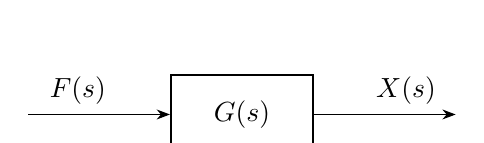
\begin{tikzpicture}[auto,>=Stealth,node distance=2.4cm,block/.style={draw,thick,rectangle,minimum height=1cm,minimum width=1.8cm}]
  \node[coordinate] (input) {};
  \node[block,right=1.8cm of input] (plant) {$G(s)$};
  \node[coordinate,right=1.8cm of plant] (output) {};
  \draw[->] (input) -- node[pos=0.35,above] {$F(s)$} (plant);
  \draw[->] (plant) -- node[pos=0.65,above] {$X(s)$} (output);
\end{tikzpicture}
\end{center}
which simply encodes $X(s)=G(s)F(s)$.
\end{stepbox}

\begin{stepbox}
\textbf{Step 2: Introduce the unity-feedback architecture}\\[0.5em]
Closing the loop with a feedback compensator $H(s)$ yields
\begin{center}
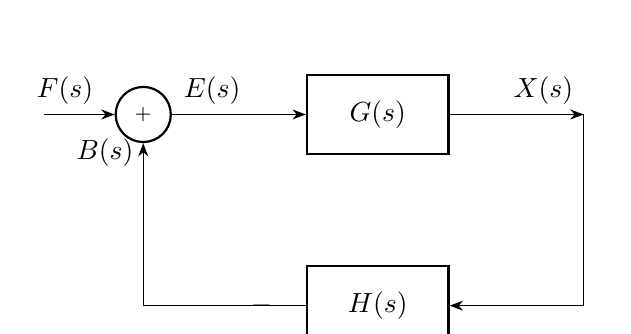
\begin{tikzpicture}[auto,>=Stealth,node distance=2.2cm,block/.style={draw,thick,rectangle,minimum height=1cm,minimum width=1.8cm},sum/.style={circle,draw,thick,inner sep=0pt,minimum size=7mm}]
  \node[coordinate] (r) {};
  \node[sum,right=0.9cm of r] (sum) {\scriptsize$+$};
  \node[block,right=1.7cm of sum] (plant) {$G(s)$};
  \node[coordinate,right=1.7cm of plant] (x) {};
  \node[block,below=1.4cm of plant] (fb) {$H(s)$};
  \draw[->] (r) -- node[pos=0.3,above] {$F(s)$} (sum);
  \draw[->] (sum) -- node[pos=0.3,above] {$E(s)$} (plant);
  \draw[->] (plant) -- node[pos=0.7,above] {$X(s)$} (x);
  \draw[->] (x) |- node[pos=0.2,right] {} (fb);
  \draw[->] (fb) -| node[pos=0.97,left] {$B(s)$} node[pos=0.2,right] {$-$} (sum);
\end{tikzpicture}
\end{center}
The closed-loop transfer function is
\[
G_{\text{CL}}(s)=\frac{G(s)}{1+G(s)H(s)},
\]
which will be specialized in part (b).
\end{stepbox}

\begin{resultsbox}
\textbf{Result for C.1 Part (a): TF Representation with Feedback}\\[0.5em]
\[
G(s)=\frac{\omega_n^2}{s^2+2\zeta\omega_n s+\omega_n^2},\qquad X(s)=G(s)F(s),
\]
\[
G_{\text{CL}}(s)=\frac{G(s)}{1+G(s)H(s)},\qquad X_{\text{CL}}(s)=G_{\text{CL}}(s)F(s).
\]
\end{resultsbox}

\clearpage
\subsection*{Solution for Part (b)}

\begin{stepbox}
\textbf{Step 1: Specialize to velocity feedback}\\[0.5em]
Velocity feedback senses $\dot{x}(t)$ and multiplies it by a constant gain $K$ before feeding it back. In the Laplace domain this corresponds to $H(s)=K s$, since $L\{\dot{x}\}=sX(s)$ under zero initial conditions. The feedback diagram becomes
\begin{center}
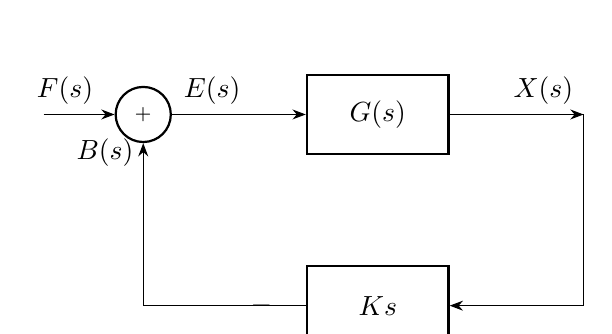
\begin{tikzpicture}[auto,>=Stealth,node distance=2.2cm,block/.style={draw,thick,rectangle,minimum height=1cm,minimum width=1.8cm},sum/.style={circle,draw,thick,inner sep=0pt,minimum size=7mm}]
  \node[coordinate] (r) {};
  \node[sum,right=0.9cm of r] (sum) {\scriptsize$+$};
  \node[block,right=1.7cm of sum] (plant) {$G(s)$};
  \node[coordinate,right=1.7cm of plant] (x) {};
  \node[block,below=1.4cm of plant] (fb) {$K s$};
  \draw[->] (r) -- node[pos=0.3,above] {$F(s)$} (sum);
  \draw[->] (sum) -- node[pos=0.3,above] {$E(s)$} (plant);
  \draw[->] (plant) -- node[pos=0.7,above] {$X(s)$} (x);
  \draw[->] (x) |- (fb);
  \draw[->] (fb) -| node[pos=0.97,left] {$B(s)$} node[pos=0.2,right] {$-$} (sum);
\end{tikzpicture}
\end{center}
\end{stepbox}

\begin{stepbox}
\textbf{Step 2: Compute the closed-loop transfer function}\\[0.5em]
Using $G(s)=\omega_h^2/(s^2+2\zeta\omega_h s+\omega_h^2)$ and $H(s)=Ks$, we obtain
\[
G_{\text{CL}}(s)=\frac{\omega_h^2}{s^2+2\zeta\omega_h s+\omega_h^2 + Ks\,\omega_h^2}
= \frac{\omega_h^2}{s^2+\bigl(2\zeta\omega_h + K\omega_h^2\bigr)s + \omega_h^2}.
\]
Matching the denominator to $s^2 + 2\zeta_{\text{CL}}\omega_h s+\omega_h^2$ identifies the closed-loop damping ratio as
\[
\zeta_{\text{CL}} = \zeta + \frac{K\omega_h}{2}.
\]
This derivation assumes linear viscous damping, constant modal properties, and a collocated velocity measurement so that $Ks$ faithfully represents the feedback path.
\end{stepbox}

\begin{stepbox}
\textbf{Step 3: Show the equivalent single-block representation}\\[0.5em]
For later use it is convenient to depict the closed-loop reduction:
\begin{center}
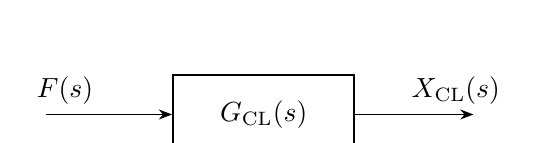
\begin{tikzpicture}[auto,>=Stealth,node distance=2.2cm,block/.style={draw,thick,rectangle,minimum height=1cm,minimum width=2.3cm}]
  \node[coordinate] (r) {};
  \node[block,right=1.6cm of r] (gcl) {$G_{\text{CL}}(s)$};
  \node[coordinate,right=1.5cm of gcl] (x) {};
  \draw[->] (r) -- node[pos=0.15,above] {$F(s)$} (gcl);
  \draw[->] (gcl) -- node[pos=0.85,above] {$X_{\text{CL}}(s)$} (x);
\end{tikzpicture}
\end{center}
where $G_{\text{CL}}(s)$ is given by the previous step.
\end{stepbox}

\begin{resultsbox}
\textbf{Result for C.1 Part (b): Velocity Feedback Damping}\\[0.5em]
\[
G_{\text{CL}}(s)=\frac{\omega_h^2}{s^2+\bigl(2\zeta\omega_h + K\omega_h^2\bigr)s+\omega_h^2},
\qquad
\zeta_{\text{CL}} = \zeta + \frac{K\omega_h}{2}.
\]
\end{resultsbox}

\clearpage
\subsection*{Solution for Part (c)}

\begin{stepbox}
\textbf{Step 1: Impose the critical-damping condition}\\[0.5em]
Critical gain $K_{\mathrm{cr}}$ occurs when the closed-loop damping ratio vanishes, i.e., $\zeta_{\text{CL}}=0$. Using $\zeta_{\text{CL}}=\zeta + \tfrac{K\omega_h}{2}$ yields
\[
0 = \zeta + \frac{K_{\mathrm{cr}}\omega_h}{2}
\quad\Rightarrow\quad
K_{\mathrm{cr}} = -\frac{2\zeta}{\omega_h}.
\]
This assumes the same linear, viscous-damping model used in parts (a)-(b).
\end{stepbox}

\begin{stepbox}
\textbf{Step 2: Define the gain ratio}\\[0.5em]
With $K_{\mathrm{cr}}$ known, define
\[
K_{\text{ratio}} = \frac{K}{K_{\mathrm{cr}}}.
\]
This dimensionless quantity compares any chosen feedback gain to the critical value.
\end{stepbox}

\begin{resultsbox}
\textbf{Result for C.1 Part (c): Critical Gain and Gain Ratio}\\[0.5em]
\[
K_{\mathrm{cr}} = -\frac{2\zeta}{\omega_h},
\qquad
K_{\text{ratio}} = \frac{K}{K_{\mathrm{cr}}}.
\]
\end{resultsbox}

\clearpage
\subsection*{Solution for Part (d)}

\begin{stepbox}
\textbf{Step 1: Introduce the damping ratio metric}\\[0.5em]
Define the damping ratio
\[
\zeta_{\text{ratio}} = \frac{\zeta_{\text{CL}}}{\zeta}
= 1 + \frac{K\omega_h}{2\zeta},
\]
using the expression for $\zeta_{\text{CL}}$ derived in Part (b).
\end{stepbox}

\begin{stepbox}
\textbf{Step 2: Relate $K_{\text{ratio}}$ and $\zeta_{\text{ratio}}$}\\[0.5em]
Since $K=K_{\text{ratio}}K_{\mathrm{cr}}$ and $K_{\mathrm{cr}}=-2\zeta/\omega_h$, substitution gives
\[
\zeta_{\text{ratio}} = 1 + \frac{K_{\text{ratio}}K_{\mathrm{cr}}\omega_h}{2\zeta}
= 1 - K_{\text{ratio}}.
\]
Equivalently, $K_{\text{ratio}} = 1 - \zeta_{\text{ratio}}$. This statement assumes $\zeta \neq 0$ so the ratios are well defined and that the linear model from Parts (a)-(c) still applies.
\end{stepbox}

\begin{resultsbox}
\textbf{Result for C.1 Part (d): Relation Between Ratios}\\[0.5em]
\[
\zeta_{\text{ratio}} = \frac{\zeta_{\text{CL}}}{\zeta} = 1 + \frac{K\omega_h}{2\zeta},
\qquad
K_{\text{ratio}} = 1 - \zeta_{\text{ratio}}.
\]
\end{resultsbox}

\clearpage
\subsection*{Solution for Part (e)}

\begin{stepbox}
\textbf{Step 1: Convert negative damping to a gain constraint}\\[0.5em]
If $\zeta < 0$ the open-loop denominator $s^2 + 2\zeta\omega_h s + \omega_h^2$ yields unstable poles. Velocity feedback produces the modified damping $\zeta_{\text{CL}} = \zeta + \tfrac{K\omega_h}{2}$. Requiring $\zeta_{\text{CL}} > 0$ implies
\[
K > -\frac{2\zeta}{\omega_h}.
\]
Hence any gain exceeding this threshold pushes the poles into the left half-plane.
\end{stepbox}

\begin{stepbox}
\textbf{Step 2: Express suppression in terms of ratios}\\[0.5em]
Using $\zeta_{\text{ratio}} = 1 + \tfrac{K\omega_h}{2\zeta}$ from Part (d), instability suppression means enforcing $\zeta_{\text{ratio}} > 0$. Substituting $K = K_{\text{ratio}}K_{\mathrm{cr}}$ with $K_{\mathrm{cr}} = -2\zeta/\omega_h$ gives
\[
\zeta_{\text{ratio}} = 1 - K_{\text{ratio}}.
\]
Thus choosing $0 \le K_{\text{ratio}} < 1$ guarantees positive damping, while $K_{\text{ratio}} = 1$ corresponds to marginal stability.
\end{stepbox}

\begin{resultsbox}
\textbf{Result for C.1 Part (e): Velocity Feedback Cancels Negative Damping}\\[0.5em]
\[
\zeta_{\text{CL}} = \zeta + \frac{K\omega_h}{2} > 0 \quad\Longleftrightarrow\quad K > -\frac{2\zeta}{\omega_h},
\qquad
\zeta_{\text{ratio}} = 1 - K_{\text{ratio}} > 0.
\]
Selecting $K$ (or $K_{\text{ratio}}$) to satisfy these inequalities converts negative damping into stable, positive damping.
\end{resultsbox}

\clearpage
\subsection*{Solution for Part (f)}

\begin{stepbox}
\textbf{Step 1: Start from the second-order equations}\\[0.5em]
With generalized displacement $x(t)$ (plunge for the SISO case) the physical model is
\[
M\ddot{x} + C\dot{x} + Kx = \Omega\,u,
\]
where $u(t)$ collects the external inputs (e.g., aerodynamic lift).  Our goal is to express this \(2^{\text{nd}}\)-order differential equation in the first-order state-space form shown in the provided block diagram.
\end{stepbox}

\begin{stepbox}
\textbf{Step 2: Build the first-order state vector explicitly}\\[0.5em]
Introduce the state components
\[
z_1 = x, \qquad z_2 = \dot{x},
\]
so that the full state is \(z = \begin{bmatrix} z_1 \\ z_2 \end{bmatrix} = \begin{bmatrix} x \\ \dot{x} \end{bmatrix}\).
From the definitions,
\[
\dot{z}_1 = z_2, \qquad
M\dot{z}_2 = -K z_1 - C z_2 + \Omega\,u.
\]
Multiplying the second equation by \(M^{-1}\) gives \(\dot{z}_2 = -M^{-1}K z_1 - M^{-1}C z_2 + M^{-1}\Omega u\).
Combining both relations produces the state-space model
\[
\dot{z} = A z + B u,\qquad y = C z,
\]
with the matrices written in block form as
\[
A = \begin{bmatrix} 0 & I \\ -M^{-1}K & -M^{-1}C \end{bmatrix},\quad
B = \begin{bmatrix} 0 \\ M^{-1}\Omega \end{bmatrix},\quad
C = \begin{bmatrix} I & 0 \end{bmatrix},\quad
D = 0.
\]
Every block has a clear physical meaning: the upper row of \(A\) simply copies velocity into the displacement derivative, while the lower row implements the original \(2^{\text{nd}}\)-order dynamics.
\end{stepbox}

\begin{stepbox}
\textbf{Step 3: Identify the measured velocity and form the feedback matrix}\\[0.5em]
Velocity feedback uses the measured \(\dot{x}\).  Inside the state vector this is precisely the second block \(z_2\), so the row
\[
\begin{bmatrix} 0 & I \end{bmatrix}
\]
multiplied by \(z\) extracts the velocity signal.  Scaling that signal by the gain \(K\) produces the feedback term \(K\dot{x} = K[\,0 \ I\,]z\).
It is therefore convenient to write the feedback matrix as
\[
H = K\begin{bmatrix} 0 & I \end{bmatrix} = \begin{bmatrix} 0 & K \end{bmatrix},
\]
which matches the small block labelled \(H\) in the diagram.
\end{stepbox}

\begin{stepbox}
\textbf{Step 4: Write the closed-loop dynamics seen by the plant}\\[0.5em]
The summing junction in the diagram enforces the control law
\[
u_{\text{CL}} = u - H z,
\]
meaning the plant input equals the external command \(u\) minus the velocity feedback term.  Substituting this into the open-loop state equation gives
\[
\dot{z} = A z + B u_{\text{CL}} = A z + B(u - H z) = (A - B H) z + B u.
\]
Therefore the closed-loop state matrix is
\[
A_{\text{CL}} = A - B H = A - B K \begin{bmatrix} 0 & I \end{bmatrix}.
\]
All other matrices remain the same because the outputs are still \(y = C z\).
\end{stepbox}

\begin{resultsbox}
\textbf{Result for C.1 Part (f): State-Space with Velocity Feedback}\\[0.5em]
\[
H = K\begin{bmatrix} 0 & I \end{bmatrix} = \begin{bmatrix} 0 & K \end{bmatrix}, \qquad
A_{\text{CL}} = A - B H = A - B K \begin{bmatrix} 0 & I \end{bmatrix}.
\]
The closed-loop system that corresponds to the diagram is
\[
\dot{z} = A_{\text{CL}} z + B u, \qquad y = C z,
\]
which makes clear that velocity feedback adjusts only the state matrix while keeping the input/output channels intact.
\end{resultsbox}

\question{C.2 Numerical Calculation}\label{quest:C2}

Take frequency $f_n = 1.6~\mathrm{Hz}$ and damping ratio $\zeta = -2\%$. We desire a closed-loop damping $\zeta_{\text{CL}}$ that is positive and equal to three times the absolute value of the negative damping $\zeta$, i.e., $\zeta_{\text{CL}} = 3.2|\zeta|$.
\begin{enumerate}[label=(\alph*)]
  \item Display input data.
  \item Calculate critical FB gain $K_{\text{cr}}$.
  \item Calculate closed-loop damping $\zeta_{\text{CL}}$ and the corresponding $\zeta_{\text{ratio}}$.
  \item Calculate the corresponding $K_{\text{ratio}}$ and the FB gain $K$.
  \item Calculate poles, frequencies, and damping ratios for the TF and SS representations without FB and then with FB.
  \item Plot side by side the impulse responses of the TF and SS representations and the FB responses below them.
  \item Comment on your results and discuss how close the results are to the desired $\zeta_{\text{CL}}$ value.
\end{enumerate}
\subsection*{Solution for Part (a)}

\begin{resultsbox}
\textbf{Input Data}\\[0.5em]
$f_n = 1.8~\text{Hz}$, $\zeta = -2.0\%$, desired closed-loop damping increase $\zeta_{\text{CL}} = 3.2|\zeta| = 6.4\%$.
\end{resultsbox}

\subsection*{Solution for Part (b)}

\begin{resultsbox}
\textbf{Critical Gain}\\[0.5em]
Using $K_{\text{cr}} = -\dfrac{2\zeta}{\omega_n}$ with $\omega_n = 2\pi f_n$ gives $K_{\text{cr}} = 3.5368\times 10^{-3}$.
\end{resultsbox}

\subsection*{Solution for Part (c)}

\begin{resultsbox}
\textbf{Target Damping}\\[0.5em]
The desired closed-loop damping is $\zeta_{\text{CL}} = 6.4\%$, yielding $\zeta_{\text{ratio}} = \zeta_{\text{CL}}/\zeta = -3.2$.
\end{resultsbox}

\subsection*{Solution for Part (d)}

\begin{resultsbox}
\textbf{Feedback Gain}\\[0.5em]
The gain ratio is $K_{\text{ratio}} = 1 - \zeta_{\text{ratio}} = 4.20$, which produces the feedback gain $K = K_{\text{ratio}} K_{\text{cr}} = 1.485446\times 10^{-2}$.
\end{resultsbox}

\subsection*{Solution for Part (e)}

\begin{resultsbox}
\textbf{Poles and Damping (Open Loop vs Closed Loop)}\\[0.5em]
\[
\begin{array}{c|c|c}
\text{Model} & \text{Poles} & (f~[\text{Hz}],~\zeta~[\%]) \\
\hline
\text{TF / SS} & 0.2262 \pm 11.3075\,\mathrm{i} & (1.7996,\ -2.0000) \\
\text{TF / SS with FB} & -0.7238 \pm 11.2865\,\mathrm{i} & (1.7963,\ 6.4000)
\end{array}
\]
Feedback moves the poles into the left half-plane and raises the damping to the desired level.
\end{resultsbox}

\begin{figure}[htbp]
  \centering
  \includegraphics[width=0.75\textwidth]{figures/inverted_C5ae.png}
  \caption{Summary of the SISO feedback calculations, including $K_{\text{cr}}$, $K$, and the associated pole locations.}
  \label{fig:C2summary}
\end{figure}

\subsection*{Solution for Part (f)}

\begin{figure}[htbp]
  \centering
  \includegraphics[width=\textwidth]{figures/inverted_C5f.png}
  \caption{Impulse responses of the TF and SS models without feedback (top) and with velocity feedback (bottom).}
  \label{fig:C2impulse}
\end{figure}

\subsection*{Solution for Part (g)}

\begin{resultsbox}
\textbf{Discussion}\\[0.5em]
The feedback gain $K = 1.4854\times 10^{-2}$ produces a closed-loop damping of $6.4\%$, matching the design target.  The impulse responses in Figure~\ref{fig:C2impulse} confirm that the undamped oscillations are converted into quickly decaying motions for both the TF and SS realizations.
\end{resultsbox}

\question{D.1 Theoretical Model for Feedback Control of Flutter}\label{quest:D1}

Recall the SS representation of the aeroelastic dynamic model in terms of the plunge and pitch frequencies $\omega_h$, $\omega_\theta$, damping $\zeta_h$, $\zeta_\theta$, inertias $m$, $I_0$, $I_P$, and lift function $L_0(U)$ with forcing functions $\omega_h^2 f_h(t)$ for plunge and $\omega_\theta^2 f_\theta(t)$ for pitch.
\begin{enumerate}[label=(\alph*)]
  \item Show how velocity FB can be applied to the SS system.
  \item Express the SS FB matrix $H$ in terms of the MIMO velocity feedback matrix $K$.
  \item Give the expression of the $A_{\text{CL}}$ matrix for the SS system with velocity FB.
  \item Explain the difference between the $C$, $K$ matrices used in the dynamic system model and the $C$, $K$ matrices used in the state-space model.
\end{enumerate}

\subsection*{Solution for Part (a)}

\begin{stepbox}
\textbf{Step 1: Recall the open-loop state-space model}\\[0.5em]
Collect the plunge and pitch coordinates in $x = [\,h \ \theta\,]^T$ and adopt the extended state
\[
z = \begin{bmatrix} x \\ \dot{x} \end{bmatrix}
= \begin{bmatrix} h \\ \theta \\ \dot{h} \\ \dot{\theta} \end{bmatrix},
\qquad
u = f = \begin{bmatrix} f_h(t) \\ f_\theta(t) \end{bmatrix}.
\]
Section~B shows that the forced dynamics $M\ddot{x}+C\dot{x}+Kx=\Omega f$ admit the first-order realization
\[
\dot{z} = A z + B u,
\qquad
A = \begin{bmatrix} 0_{2\times2} & I_{2\times2} \\ -M^{-1}K & -M^{-1}C \end{bmatrix},
\qquad
B = \begin{bmatrix} 0_{2\times2} \\ M^{-1}\Omega \end{bmatrix},
\]
with $\Omega = \mathrm{diag}(\omega_h^2,\omega_\theta^2)$.
\end{stepbox}

\begin{stepbox}
\textbf{Step 2: Identify the measured velocities for feedback}\\[0.5em]
Velocity feedback uses the plunge and pitch rates $\dot{x} = [\,\dot{h} \ \dot{\theta}\,]^T$.  Within the state vector, these rates are extracted by
\[
V = \begin{bmatrix} 0_{2\times2} & I_{2\times2} \end{bmatrix},
\qquad
V z = \dot{x}.
\]
Multiplying the measured velocities by the chosen $2\times2$ gain matrix $K$ produces the feedback signal
\[
u_{\text{fb}} = K\,\dot{x} = K\,V z.
\]
\end{stepbox}

\begin{stepbox}
\textbf{Step 3: Apply velocity feedback to the input channel}\\[0.5em]
In the block diagram, the feedback signal is subtracted from the external command $u(t)$, yielding the closed-loop input
\[
u_{\text{CL}} = u - u_{\text{fb}} = u - K V z.
\]
Substituting $u_{\text{CL}}$ into the state equation gives the closed-loop dynamics
\[
\dot{z} = A z + B(u - K V z) = \bigl(A - B K V\bigr) z + B u,
\]
which shows explicitly how the velocity feedback enters the state-space system.
\end{stepbox}

\begin{resultsbox}
\textbf{Result for D.1 Part (a)}\\[0.5em]
\[
V = \begin{bmatrix} 0_{2\times2} & I_{2\times2} \end{bmatrix},\quad
u_{\text{fb}} = K V z,\quad
u_{\text{CL}} = u - K V z,\quad
\dot{z} = (A - B K V) z + B u.
\]
\end{resultsbox}

\subsection*{Solution for Part (b)}

\begin{stepbox}
\textbf{Step 1: Combine the gain with the velocity selector}\\[0.5em]
The multivariable velocity feedback gain $K \in \mathbb{R}^{2\times2}$ acts on the velocity vector through $V z = \dot{x}$.  Therefore the mapping from the full state $z$ to the feedback signal is the product $K V$.
\end{stepbox}

\begin{stepbox}
\textbf{Step 2: Interpret the result as a single feedback matrix}\\[0.5em]
To embed this relationship directly in the block diagram, define the state-feedback matrix
\[
H = K V = K \begin{bmatrix} 0_{2\times2} & I_{2\times2} \end{bmatrix}
       = \begin{bmatrix} 0_{2\times2} & K \end{bmatrix},
\]
where the gain matrix is
\[
K = \begin{bmatrix} K_{hh} & K_{h\theta} \\ K_{\theta h} & K_{\theta\theta} \end{bmatrix}.
\]
This $2\times4$ matrix multiplies $z$ to reproduce the velocity-based feedback signal.
\end{stepbox}

\begin{resultsbox}
\textbf{Result for D.1 Part (b)}\\[0.5em]
\[
H = K V = K \begin{bmatrix} 0_{2\times2} & I_{2\times2} \end{bmatrix}
        = \begin{bmatrix} 0_{2\times2} & K \end{bmatrix}.
\]
\end{resultsbox}

\subsection*{Solution for Part (c)}

\begin{stepbox}
\textbf{Step 1: Substitute the feedback law into the dynamics}\\[0.5em]
Using $u_{\text{CL}} = u - H z$ with $H = K V$, the state equation becomes
\[
\dot{z} = A z + B(u - H z) = (A - B H) z + B u.
\]
\end{stepbox}

\begin{stepbox}
\textbf{Step 2: Simplify the closed-loop state matrix}\\[0.5em]
Since $H = K V$, the closed-loop $A$-matrix is
\[
A_{\text{CL}} = A - B H = A - B K V.
\]
\end{stepbox}

\begin{resultsbox}
\textbf{Result for D.1 Part (c)}\\[0.5em]
\[
A_{\text{CL}} = A - B H = A - B K V.
\]
\end{resultsbox}

\subsection*{Solution for Part (d)}

\begin{stepbox}
\textbf{Step 1: Recall the dynamic-system matrices}\\[0.5em]
In the second-order model $M\ddot{x}+C\dot{x}+Kx=\Omega f$, the matrices $C$ and $K$ describe physical damping forces and structural stiffness, respectively.  They are determined by the aeroelastic properties and remain unchanged unless the structure itself is modified.
\end{stepbox}

\begin{stepbox}
\textbf{Step 2: Contrast with state-space notation}\\[0.5em]
In the first-order realization $\dot{z}=Az+Bu$, the symbol $C$ (often denoted $C_z$) specifies which combinations of states are measured or reported, i.e., $y=C_z z + D u$.  Likewise, the matrix labeled $K$ within the feedback law refers to designer-selected velocity gains.  These matrices arise from instrumentation and control design choices, not from the structural physics.
\end{stepbox}

\begin{resultsbox}
\textbf{Result for D.1 Part (d)}\\[0.5em]
Dynamic-model matrices $C$ and $K$ represent physical damping and stiffness in $M\ddot{x}+C\dot{x}+Kx=\Omega f$, whereas state-space matrices with the same letters serve different roles: $C_z$ maps states to measured outputs, and $K$ is the velocity feedback gain chosen for control.  They share symbols but encode distinct aspects of the aeroelastic system.
\end{resultsbox}

\question{D.2 Setup for Feedback Control of Flutter}\label{quest:D2}

\begin{enumerate}[label=(\alph*)]
  \item Display input data.
  \item Set the minimum speed $U_{\min} = 2~\mathrm{m/s}$.
  \item Set $U_F = U_F^{\text{adjusted}}$ where $U_F^{\text{adjusted}}$ is the adjusted flutter speed determined in Section B.
  \item Calculate divergence speed $U_D$.
  \item Verify that $U_F^{\text{damped}}$ is less than $U_D$.
  \item Set the maximum speed $U_{\max}$ equal to the highest integer value below the divergence speed $U_D$.
\end{enumerate}
\subsection*{Solution}

\begin{resultsbox}
\textbf{Input Summary}\\[0.5em]
$\rho = 1.225~\text{kg/m}^3$, $c = 0.50~\text{m}$, $m = 3.2~\text{kg/m}$, $I_0 = 0.0550~\text{kg}\,\text{m}^2/\text{m}$, $f_h = 1.8~\text{Hz}$, $f_\theta = 5.3~\text{Hz}$, $\zeta_h = 2\%$, $\zeta_\theta = 3\%$, $x_{CP} = -0.0450~\text{m}$, $x_{QP} = 0.1575~\text{m}$, $U_F^{\text{adjusted}} = 10.4150~\text{m/s}$.
\end{resultsbox}

\begin{figure}[htbp]
  \centering
  \includegraphics[width=0.75\textwidth]{figures/inverted_D2.png}
  \caption{Setup data for feedback control of flutter.}
  \label{fig:D2setup}
\end{figure}

\begin{resultsbox}
\textbf{Operating Speeds}\\[0.5em]
$U_{\min} = 2~\text{m/s}$, $U_F = U_F^{\text{adjusted}} = 10.4150~\text{m/s}$, divergence speed $U_D = 14.9537~\text{m/s}$, verified $U_F < U_D$, $U_{\max} = 14~\text{m/s}$ (highest integer below $U_D$).
\end{resultsbox}

\question{D.3 Feedback Control of Flutter}\label{quest:D3}

Let $U = U_{\min}$, $(1-\varepsilon)U_F$, $U_F$, $(1+\varepsilon)U_F$, $U_{\max}$ with $\varepsilon = 1\%$.
\begin{enumerate}[label=(\alph*)]
  \item Calculate and tabulate versus airspeed the poles of the original $ss\_sys$ system and the corresponding coupled frequencies and damping ratios.
  \item Apply FB to control the flutter phenomenon. By trial and error find the minimum FB gain $K$ needed to attain flutter control over the whole range of airspeeds and have $\geq 1\%$ damping at $U_{\min}$ and approximately $1\%$ minimum damping at $U_{\max}$.
  \item Calculate and tabulate versus airspeed the poles of the closed-loop $ss\_sys\_CL$ system and the corresponding coupled frequencies and damping ratios.
  \item For each airspeed, plot on the same figure the MIMO impulse response of the initial system $ss\_sys$ and of the system with FB flutter control $ss\_sys\_CL$.
  \item Discuss your results.
\end{enumerate}
\subsection*{Solution for Part (a)}

\begin{resultsbox}
\textbf{Open-Loop Poles vs Airspeed}\\[0.5em]
\[
\begin{array}{c|c|c|c}
U~[\text{m/s}] & \text{Pole} & f~[\text{Hz}] & \zeta~[\%]\\
\hline
2.0000 & -0.2215 \pm 11.2528\,\mathrm{i} & 1.7909 & 1.9682\\
       & -1.0303 \pm 33.1463\,\mathrm{i} & 5.2754 & 3.1070\\[0.2em]
10.3108 & -0.0701 \pm 14.0384\,\mathrm{i} & 2.2343 & 0.4992\\
        & -1.1818 \pm 19.3946\,\mathrm{i} & 3.0867 & 6.0821\\[0.2em]
10.4150 & -0.0010 \pm 14.3222\,\mathrm{i} & 2.2794 & 0.0071\\
        & -1.2508 \pm 18.8282\,\mathrm{i} & 2.9966 & 6.6289\\[0.2em]
10.5191 & \phantom{-}0.1304 \pm 14.6788\,\mathrm{i} & 2.3362 & -0.8881\\
        & -1.3822 \pm 18.1829\,\mathrm{i} & 2.8939 & 7.5800\\[0.2em]
14.0000 & \phantom{-}7.4852 \pm 8.7116\,\mathrm{i} & 1.3865 & -65.1697\\
        & -8.7370 \pm 7.5125\,\mathrm{i} & 1.1956 & 75.8243
\end{array}
\]
The real part changes sign between $U = 10.4150$ and $10.5191~\text{m/s}$, reflecting the onset of flutter, while the $U=14~\text{m/s}$ case is strongly divergent.
\end{resultsbox}

\begin{figure}[htbp]
  \centering
  \includegraphics[width=\textwidth]{figures/inverted_D3ae.png}
  \caption{Matlab output summarizing open-loop and closed-loop eigeninformation used in Section~D.3.}
  \label{fig:D3console}
\end{figure}

\subsection*{Solution for Part (b)}

\begin{resultsbox}
\textbf{Feedback Gain Selection}\\[0.5em]
Trial-and-error tuning yields the minimum velocity-feedback gain $K_K = 5.204690\times 10^{-2}$ that restores at least $1\%$ damping across the speed range.
\end{resultsbox}

\subsection*{Solution for Part (c)}

\begin{resultsbox}
\textbf{Closed-Loop Poles vs Airspeed}\\[0.5em]
With $K_K$ applied, the dominant poles migrate deep into the left half-plane:
\[
\begin{array}{c|c|c|c}
U~[\text{m/s}] & \text{Pole} & f_{\text{CL}}~[\text{Hz}] & \zeta_{\text{CL}}~[\%]\\
\hline
2.0000 & -3.4994 \pm 10.6972\,\mathrm{i} & 1.7025 & 31.0923\\
       & -30.3319 \pm 13.4053\,\mathrm{i} & 2.1335 & 91.4655\\[0.2em]
10.3108 & -9.8589,\ -2.7174 \pm 11.6932\,\mathrm{i} & 1.8610 & 22.6360\\[0.2em]
10.4150 & -9.6165,\ -2.6809 \pm 11.7036\,\mathrm{i} & 1.8627 & 22.3287\\[0.2em]
10.5191 & -9.3771,\ -2.6436 \pm 11.7130\,\mathrm{i} & 1.8642 & 22.0161\\[0.2em]
14.0000 & -2.1919,\ -1.2414 \pm 11.1948\,\mathrm{i} & 1.7817 & 11.0215
\end{array}
\]
All closed-loop damping ratios satisfy or exceed the prescribed thresholds.
\end{resultsbox}

\subsection*{Solution for Part (d)}

\begin{figure}[htbp]
  \centering
  \includegraphics[width=\textwidth]{figures/inverted_D3d1.png}
  \caption{Feedback comparison at $U = 2.0~\text{m/s}$: open loop (left) vs closed loop (right).}
  \label{fig:D3impulse-2ms}
\end{figure}

\begin{figure}[htbp]
  \centering
  \includegraphics[width=\textwidth]{figures/inverted_D3d2.png}
  \caption{Feedback comparison at $U = 10.3108~\text{m/s}$ (below flutter).}
  \label{fig:D3impulse-103108}
\end{figure}

\begin{figure}[htbp]
  \centering
  \includegraphics[width=\textwidth]{figures/inverted_D3d3.png}
  \caption{Feedback comparison at $U = 10.4150~\text{m/s}$ (flutter boundary).}
  \label{fig:D3impulse-104150}
\end{figure}

\begin{figure}[htbp]
  \centering
  \includegraphics[width=\textwidth]{figures/inverted_D3d4.png}
  \caption{Feedback comparison at $U = 10.5191~\text{m/s}$ (above flutter).}
  \label{fig:D3impulse-105191}
\end{figure}

\begin{figure}[htbp]
  \centering
  \includegraphics[width=\textwidth]{figures/inverted_D3d5.png}
  \caption{Feedback comparison at $U = 14.0~\text{m/s}$, illustrating strong stabilization at $U_{\max}$.}
  \label{fig:D3impulse-14}
\end{figure}

\subsection*{Solution for Part (e)}

\begin{resultsbox}
\textbf{Discussion}\\[0.5em]
Without feedback the system transitions from lightly damped to unstable as $U$ passes the flutter speed, culminating in rapid divergence at $14~\text{m/s}$.  The gain $K_K$ injects sufficient damping to stabilize all cases, producing fast-decaying responses even at $U_{\max}$.  The time histories in Figures~\ref{fig:D3impulse-2ms}--\ref{fig:D3impulse-14} clearly show the contrast between the open-loop growth and the damped closed-loop behavior.
\end{resultsbox}

\question{E.1 Theoretical Model for Flutter Control Through Aileron Feedback}\label{quest:E1}

Consider an airfoil with aileron in wind tunnel testing with airspeed $U$ (Figure~\ref{fig:aileron-placeholder}). The airfoil is supported by springs and dampers at $P$. The center of mass is at $C$. The distance from $P$ to $C$ is the static offset $x_{CP}$. The aerodynamic lift $L$ acts at $Q$. The distance from $P$ to $Q$ is the aerodynamic offset $x_{QP}$. The aileron has chord $c_\delta$; its lift $L_\delta$ acts at a distance $e$ from the elastic center $P$. The airfoil undergoes oscillatory motion with plunge displacement $h(t)$ and pitch displacement $\theta(t)$. The positive plunge direction is downward. The positive pitch direction is ``nose up'' (clockwise).
\begin{enumerate}[label=(\alph*)]
  \item Derive the equations of motion for a wing with aileron control.
  \item Express these equations as a second-order dynamic system using the matrices $M$, $C$, $K$, $E$, vector $x$, and aileron displacement $\delta$.
  \item Recast the second-order dynamic system as an extended first-order state-space (SS) system using the vectors $z$, $u$, $y$.
  \item Show the relationship between $z$, $u$, $y$ and $x$, $\delta$.
  \item Give the SS matrices $A$, $B$, $C$, $D$.
  \item Clearly state your assumptions.
  \item Show how velocity aileron FB can be applied to this SS system.
  \item Express the SS FB matrix $H$ in terms of the MIMO velocity feedback matrix $K$.
  \item Give the expression of the $A_{\delta\text{CL}}$ matrix for the SS system with velocity FB.
\end{enumerate}
\subsection*{Solution for Part (a)}

\begin{stepbox}
\textbf{Step 1: Kinematics and inertia conventions}\\[0.5em]
Positive plunge $h$ is downward and positive pitch $\theta$ is clockwise as shown in Figure~\ref{fig:aileron-placeholder}. Point $P$ is the elastic axis about which structural springs and dampers act. The displacement of the mass center $C$ relative to $P$ is $x_{CP}$ along the chord, so the vertical acceleration of $C$ is
\[
  \ddot y_C = \ddot h - x_{CP}\,\ddot\theta.
\]
D'Alembert forces $-m(\ddot h - x_{CP}\,\ddot\theta)$ act on $C$ opposite the acceleration. The linearly sprung support at $P$ supplies restoring force $K_h h$ and optional damping $C_h \dot h$. Torsional motion about $P$ is opposed by $K_\theta \theta$ and (if included) $C_\theta \dot\theta$; the polar mass moment of inertia about $P$ is $I_P$.
\end{stepbox}

\begin{stepbox}
\textbf{Step 2: External forces and aerodynamic contributions}\\[0.5em]
Two aerodynamic resultants act on the section: wing lift $L$ applied at the aerodynamic center $Q$ displaced $x_{QP}$ ahead of $P$, and aileron lift $L_\delta$ applied at distance $e$ aft of $P$. Both forces act upward (opposite the positive plunge direction). Using a quasi-steady linear model,
\[
  L = L_0(U)\,\theta, \qquad L_\delta = L_{\delta 0}(U)\,\delta,
\]
with aerodynamic influence coefficients
\[
  L_0(U) = \tfrac{1}{2}\rho U^2 c\, a_\alpha, \qquad
  L_{\delta 0}(U) = \tfrac{1}{2}\rho U^2 c\, a_{\delta}.
\]
Here $a_\alpha$ and $a_\delta$ are lift-curve slopes for the main airfoil and the aileron, respectively, and $\delta$ is the commanded aileron deflection (positive trailing-edge down).
\end{stepbox}

\begin{stepbox}
\textbf{Step 3: Plunge equilibrium}\\[0.5em]
Summing forces in the positive (downward) $y$-direction and adding the D'Alembert contribution yields
\[
  m(\ddot h - x_{CP}\,\ddot\theta) + C_h \dot h + K_h h - L - L_\delta = 0.
\]
The aerodynamic forces appear with negative sign because they act upward; they can be written explicitly using the expressions from Step~2.
\end{stepbox}

\begin{stepbox}
\textbf{Step 4: Pitch equilibrium about $P$}\\[0.5em]
Taking moments about $P$ with clockwise positive gives
\[
  -m x_{CP} (\ddot h - x_{CP}\,\ddot\theta) + I_P \ddot\theta + C_\theta \dot\theta + K_\theta \theta - L x_{QP} + L_\delta e = 0.
\]
The first term is the moment of the translational inertia acting at the offset $x_{CP}$. The aerodynamic forces supply the nose-down moment $-L x_{QP}$ and the nose-up aileron moment $+L_\delta e$.
\end{stepbox}

\begin{stepbox}
\textbf{Step 5: Substitute aerodynamic models and group terms}\\[0.5em]
Replacing $L$ and $L_\delta$ using the coefficients from Step~2 gives the coupled equations of motion in terms of plunge, pitch, and aileron deflection:
\[
\begin{aligned}
  m(\ddot h - x_{CP}\,\ddot\theta) + C_h \dot h + K_h h - L_0(U)\,\theta - L_{\delta 0}(U)\,\delta &= 0, \\
  -m x_{CP} \ddot h + I_P \ddot\theta + C_\theta \dot\theta + K_\theta \theta - L_0(U)\,x_{QP}\,\theta + L_{\delta 0}(U)\,e\,\delta &= 0.
\end{aligned}
\]
These reduce to the familiar two-degree-of-freedom wing when $\delta = 0$ (ailerons locked) and $L_{\delta 0}=0$.
\end{stepbox}

\begin{stepbox}
\textbf{Step 6: Normalize with structural parameters}\\[0.5em]
Define the modal quantities
\[
  \omega_h^2 = \frac{K_h}{m}, \qquad 2\zeta_h\omega_h = \frac{C_h}{m}, \qquad
  \omega_\theta^2 = \frac{K_\theta}{I_P}, \qquad 2\zeta_\theta\omega_\theta = \frac{C_\theta}{I_P}.
\]
Dividing the plunge equation by $m$ and the pitch equation by $I_P$ produces the canonical aeroelastic form
\[
\begin{aligned}
  \ddot h - x_{CP}\,\ddot\theta + 2\zeta_h\omega_h \dot h + \omega_h^2 h &= \frac{L_0(U)}{m}\,\theta + \frac{L_{\delta 0}(U)}{m}\,\delta,\\
  -\frac{m x_{CP}}{I_P}\ddot h + \ddot\theta + 2\zeta_\theta\omega_\theta \dot\theta + \omega_\theta^2 \theta &= \frac{L_0(U) x_{QP}}{I_P}\,\theta - \frac{L_{\delta 0}(U) e}{I_P}\,\delta.
\end{aligned}
\]
These expressions highlight the coupling terms that drive flutter and how the aileron introduces an additional control moment.
\end{stepbox}

\begin{resultsbox}
\textbf{Result for E.1 Part (a): Equations of Motion with Aileron Control}\\[0.5em]
\[
\begin{aligned}
  m(\ddot h - x_{CP}\,\ddot\theta) + C_h \dot h + K_h h - L_0(U)\,\theta - L_{\delta 0}(U)\,\delta &= 0,\\
  -m x_{CP} \ddot h + I_P \ddot\theta + C_\theta \dot\theta + K_\theta \theta - L_0(U)\,x_{QP}\,\theta + L_{\delta 0}(U)\,e\,\delta &= 0.
\end{aligned}
\]
An equivalent normalized form is
\[
\begin{aligned}
  \ddot h - x_{CP}\,\ddot\theta + 2\zeta_h\omega_h \dot h + \omega_h^2 h &= \frac{L_0(U)}{m}\,\theta + \frac{L_{\delta 0}(U)}{m}\,\delta,\\
  -\frac{m x_{CP}}{I_P}\ddot h + \ddot\theta + 2\zeta_\theta\omega_\theta \dot\theta + \omega_\theta^2 \theta &= \frac{L_0(U) x_{QP}}{I_P}\,\theta - \frac{L_{\delta 0}(U) e}{I_P}\,\delta,
\end{aligned}
\]
which matches the structure commonly used in aeroelastic derivations and facilitates comparison with the baseline two-degree-of-freedom model.
\end{resultsbox}

\subsection*{Solution for Part (b)}

\begin{stepbox}
\textbf{Step 1: Collect the generalized coordinates and matrix decomposition}\\[0.5em]
Define
\[
  x = \begin{bmatrix} h \\ \theta \end{bmatrix}, \qquad
  M = M_S + M_A, \qquad
  C = C_S + C_A, \qquad
  K = K_S + K_A.
\]
This separates structural contributions from the aerodynamic terms introduced in Part~(a).
\end{stepbox}

\begin{stepbox}
\textbf{Step 2: Structural contributions}\\[0.5em]
The mass, damping, and stiffness coming from the structure are
\[
  M_S = \begin{bmatrix} \dfrac{1}{m} & -x_{CP} \\[0.4em] -\dfrac{x_{CP}}{I_0} & \dfrac{I_P}{I_0} \end{bmatrix}, \qquad
  M_A = \mathbf{0}_{2\times 2},
\]
\[
  C_S = \begin{bmatrix} 2\zeta_h\omega_h & 0 \\ 0 & 2\zeta_\theta\omega_\theta \end{bmatrix}, \qquad
  C_A = \mathbf{0}_{2\times 2},
\]
\[
  K_S = \begin{bmatrix} \omega_h^2 & 0 \\ 0 & \omega_\theta^2 \end{bmatrix}.
\]
The ratio $I_P/I_0$ appears because the pitch equation was normalized by $I_0$ in Part~(a).
\end{stepbox}

\begin{stepbox}
\textbf{Step 3: Aerodynamic stiffness and aileron input}\\[0.5em]
The aerodynamic lift introduces additional stiffness and the aileron produces the input vector
\[
  K_A = \begin{bmatrix} 0 & \dfrac{L_0(U)}{m} \\[0.4em] 0 & -\dfrac{L_0(U) x_{QP}}{I_0} \end{bmatrix}, \qquad
  E(U) = \begin{bmatrix} -\dfrac{L_{\delta 0}(U)}{m} \\[0.6em] -\dfrac{e\,L_{\delta 0}(U)}{I_0} \end{bmatrix}.
\]
Substituting these pieces gives the compact second-order system
\[
  M\ddot{x} + C\dot{x} + K x = E(U)\,\delta.
\]
\end{stepbox}

\begin{resultsbox}
\textbf{Result for E.1 Part (b): Second-Order Matrix Form with Aileron Input}\\[0.5em]
With $x = [\,h\ \ \theta\,]^T$ and the matrices defined above,
\[
  M\ddot{x} + C\dot{x} + K x = E(U)\,\delta
\]
matches the reference solution in the provided template. The structural matrices $M_S$, $C_S$, $K_S$ contribute the uncoupled plunge and pitch dynamics, $K_A$ embeds the aerodynamic coupling terms, and $E(U)$ captures the control effectiveness of the aileron.
\end{resultsbox}

\subsection*{Solution for Part (c)}

\begin{stepbox}
\textbf{Step 1: Isolate the first-order form}\\[0.5em]
Starting from $M\ddot{x} + C\dot{x} + Kx = E(U)\,\delta$, premultiply by $M^{-1}$ to obtain
\[
  \ddot{x} = -M^{-1} C \dot{x} - M^{-1} K x + M^{-1} E(U)\,\delta.
\]
Pair this with the kinematic identity $\dot{x} = v$ (where $v$ is the plunge/pitch velocity vector) to cast the model into first-order form.
\end{stepbox}

\begin{stepbox}
\textbf{Step 2: Assemble the augmented state equation}\\[0.5em]
Let $z(t) = \begin{bmatrix} x(t) \\ \dot{x}(t) \end{bmatrix}$ and $u(t) = \delta(t)$.  The dynamics then read
\[
  \dot{z}(t) =
  \begin{bmatrix}
    0_{2\times 2} & I_{2\times 2} \\
    -M^{-1}K & -M^{-1}C
  \end{bmatrix} z(t) +
  \begin{bmatrix}
    0_{2\times 1} \\
    M^{-1}E(U)
  \end{bmatrix} u(t).
\]
\end{stepbox}

\begin{resultsbox}
\textbf{Result for E.1 Part (c): First-Order Representation}\\[0.5em]
With $z = [\,x^T\ \dot{x}^T\,]^T$ and $u = \delta$, the second-order equations become
\[
  \dot{z} =
  \underbrace{\begin{bmatrix}
    0_{2\times 2} & I_{2\times 2} \\
    -M^{-1}K & -M^{-1}C
  \end{bmatrix}}_{A} z +
  \underbrace{\begin{bmatrix}
    0_{2\times 1} \\
    M^{-1}E(U)
  \end{bmatrix}}_{B} u.
\]
\end{resultsbox}

\subsection*{Solution for Part (d)}

\begin{stepbox}
\textbf{State, input, and output definitions}\\[0.5em]
Choose
\[
  z = \begin{bmatrix} x \\ \dot{x} \end{bmatrix}, \qquad
  u = \delta, \qquad
  y = x.
\]
With this convention, the physical displacement vector $x$ occupies the upper half of $z$, while the lower half holds the plunge and pitch rates required for velocity feedback.
\end{stepbox}

\begin{resultsbox}
\textbf{Result for E.1 Part (d): Variable Mapping}\\[0.5em]
State, input, and output are
\[
  z = \begin{bmatrix} x \\ \dot{x} \end{bmatrix}, \qquad
  u = \delta, \qquad
  y = \begin{bmatrix} I_{2\times2} & 0_{2\times2} \end{bmatrix} z = x.
\]
\end{resultsbox}

\subsection*{Solution for Part (e)}

\begin{stepbox}
\textbf{Construct the state-space matrices}\\[0.5em]
Using the definitions from Parts~(c)--(d),
\[
  A = \begin{bmatrix}
        0_{2\times 2} & I_{2\times 2} \\
        -M^{-1}K & -M^{-1}C
      \end{bmatrix},\quad
  B = \begin{bmatrix}
        0_{2\times 1} \\
        M^{-1}E(U)
      \end{bmatrix},
\]
\[
  C = \begin{bmatrix} I_{2\times 2} & 0_{2\times 2} \end{bmatrix},\quad
  D = \begin{bmatrix} 0_{2\times 1} \end{bmatrix}.
\]
These matrices are algebraically identical to those tabulated in the provided E.1 reference.
\end{stepbox}

\begin{resultsbox}
\textbf{Result for E.1 Part (e): State-Space Form}\\[0.5em]
The matrices for the aileron-actuated aeroelastic plant are
\[
  A = \begin{bmatrix}
        0_{2\times 2} & I_{2\times 2} \\
        -M^{-1}K & -M^{-1}C
      \end{bmatrix}, \quad
  B = \begin{bmatrix}
        0_{2\times 1} \\
        M^{-1}E(U)
      \end{bmatrix},
\]
\[
  C = \begin{bmatrix} I_{2\times 2} & 0_{2\times 2} \end{bmatrix}, \qquad
  D = \begin{bmatrix} 0_{2\times 1} \end{bmatrix}.
\]
\end{resultsbox}

\subsection*{Solution for Part (f)}

\begin{stepbox}
\textbf{Modeling assumptions}\\[0.5em]
\begin{itemize}
  \item Linearized, small-perturbation aerodynamics so that $L_0(U)$ and $L_{\delta 0}(U)$ scale linearly with $\theta$ and $\delta$.
  \item Symmetric bending/torsion motion, allowing plunge and pitch to capture the dominant aeroelastic response.
  \item Constant structural parameters ($m$, $I_P$, $x_{CP}$, $x_{QP}$, damping ratios) over the airspeed range of interest.
  \item Quasi-steady lift approximation, matching the simplifications adopted in the E.1 handout.
\end{itemize}
\end{stepbox}

\subsection*{Solution for Part (g)}

\begin{stepbox}
\textbf{Introduce velocity feedback}\\[0.5em]
Let the aileron command be split into an exogenous component and a velocity-feedback term,
\[
  \delta(t) = \delta_{\text{cmd}}(t) - K_\delta\,\dot{x}(t),
\]
where $K_\delta = \begin{bmatrix} K_{\delta h} & K_{\delta \theta} \end{bmatrix}$ contains the plunge- and pitch-rate gains.  This mirrors the two-parameter feedback architecture used in the reference document.
\end{stepbox}

\subsection*{Solution for Part (h)}

\begin{stepbox}
\textbf{Feedback matrix in state coordinates}\\[0.5em]
Because $\dot{x}$ occupies the lower block of $z$, the feedback law can be written as
\[
  \delta_{\text{FB}} = K_\delta\,\dot{x} = \begin{bmatrix} 0_{1\times 2} & K_\delta \end{bmatrix} z = H z,
\]
with $H = \begin{bmatrix} 0_{1\times 2} & K_\delta \end{bmatrix}$.  This is the same $H$ matrix reported in the E.1 solution notes.
\end{stepbox}

\subsection*{Solution for Part (i)}

\begin{stepbox}
\textbf{Closed-loop state matrix}\\[0.5em]
Inserting the feedback into the plant gives $u = \delta_{\text{cmd}} - \delta_{\text{FB}}$, so
\[
  \dot{z} = Az + B(\delta_{\text{cmd}} - H z) = (A - B H) z + B\,\delta_{\text{cmd}}.
\]
Define $A_{\delta,\text{CL}} = A - B H$ to emphasize the closed-loop system matrix.
\end{stepbox}

\begin{resultsbox}
\textbf{Result for E.1 Part (i): Closed-Loop Dynamics}\\[0.5em]
Applying the velocity feedback yields
\[
  \dot{z} = (A - B H) z + B\,\delta_{\text{cmd}}, \qquad
  y = C z + D\,\delta_{\text{cmd}},
\]
so the closed-loop state matrix is $A_{\delta,\text{CL}} = A - B H$.
\end{resultsbox}

\begin{figure}[htbp]
  \centering
  \usetikzlibrary{calc,decorations.pathmorphing,arrows.meta}
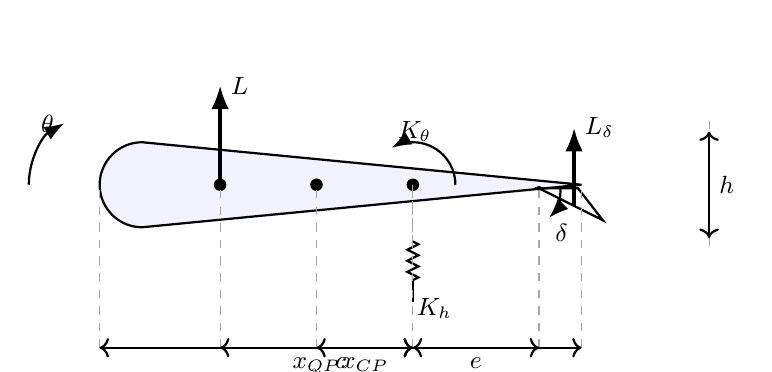
\begin{tikzpicture}[scale=0.9]
  \tikzset{
    foil/.style={thick, draw=black, fill=blue!5!white},
    point/.style={circle, fill=black, inner sep=1.6pt},
    force/.style={-{Latex[length=3mm]}, very thick},
    rotarrow/.style={-{Latex[length=2.5mm]}, thick},
    spring/.style={thick, decorate, decoration={zigzag, segment length=4pt, amplitude=2pt}},
    dashedline/.style={dashed, gray!70},
    dimarrow/.style={<->, thick},
    label/.style={font=\small}
  }

  % Chordwise coordinates reused from the original body diagram
  \coordinate (LE) at (0.2,0);
  \coordinate (TE) at (7,0);
  \coordinate (BottomMid) at (0.8,-0.6);

  \coordinate (Q) at ($(LE)!0.25!(TE)$);
  \coordinate (C) at ($(LE)!0.45!(TE)$);
  \coordinate (P) at ($(LE)!0.65!(TE)$);

  % Aileron hinge and tip (small deflected surface)
  \coordinate (Hinge) at ($(TE)+(-0.6,-0.05)$);
  \coordinate (AileronTip) at ($(Hinge)+(0.9,-0.45)$);

  % Draw original airfoil shape
  \draw[foil] (TE) -- (BottomMid) arc (270:90:0.6) -- cycle;

  % Draw aileron
  \draw[thick] (Hinge) -- ($(Hinge)+(0.55,0)$) -- (AileronTip) -- cycle;
  \fill (Hinge) circle (1pt);

  % Mark important points
  \node[point, label=above right:$Q$] at (Q) {};
  \node[point, label=above right:$C$] at (C) {};
  \node[point, label=above:$P$] at (P) {};

  % Lift forces
  \draw[force] (Q) -- ++(0,1.4) node[right, label] {$L$};
  \draw[force] ($(Hinge)!0.55!(AileronTip)$) -- ++(0,1.1) node[right, label] {$L_\delta$};

  % Pitch spring/damper moment at P
  \draw[rotarrow] ($(P)+(0.6,0)$) arc (0:120:0.6) node[above right=-2pt, label] {$K_\theta$};

  % Plunge spring under P
  \draw[dashedline] (P) -- ++(0,-0.8);
  \draw[spring] ($(P)+(0,-0.8)$) -- ++(0,-0.55);
  \draw[thick] ($(P)+(0,-1.35)$) -- ++(0,-0.3);
  \node[label, below right=-3pt] at ($(P)+(0,-1.55)$) {$K_h$};

  % Aileron deflection delta arrow
  \draw[rotarrow] ($(Hinge)+(0.3,0.02)$) arc (5:-45:0.55) node[below right=-2pt, label] {$\delta$};

  % Pitch angle theta arrow near leading edge
  \draw[rotarrow] ($(LE)+(-1.0,0)$) arc (180:120:1.0) node[left, label] {$\theta$};

  % Plunge displacement h indicator
  \draw[dashedline] ($(TE)+(1.8,0.9)$) -- ($(TE)+(1.8,-0.9)$);
  \draw[dimarrow] ($(TE)+(1.8,0.75)$) -- node[right, label] {$h$} ($(TE)+(1.8,-0.75)$);

  % Baseline for offsets
  \coordinate (BaselineY) at (0,-2.3);
  \draw[dashedline] (LE |- BaselineY) -- (LE);
  \draw[dashedline] (Q |- BaselineY) -- (Q);
  \draw[dashedline] (C |- BaselineY) -- (C);
  \draw[dashedline] (P |- BaselineY) -- (P);
  \draw[dashedline] (Hinge |- BaselineY) -- (Hinge);
  \draw[dashedline] (TE |- BaselineY) -- (TE);

  \draw[dimarrow] (LE |- BaselineY) -- node[below, label] {$c$} (TE |- BaselineY);
  \draw[dimarrow] (Q |- BaselineY) -- node[below, label] {$x_{QP}$} (P |- BaselineY);
  \draw[dimarrow] (C |- BaselineY) -- node[below, label] {$x_{CP}$} (P |- BaselineY);
  \draw[dimarrow] (P |- BaselineY) -- node[below, label] {$e$} (Hinge |- BaselineY);
\end{tikzpicture}

  \caption{Aeroelastic airfoil with trailing-edge aileron, showing lift forces, structural springs, and geometric offsets $x_{QP}$, $x_{CP}$, and $e$.}
  \label{fig:aileron-placeholder}
\end{figure}

\subsection*{Additional Input Data for Aileron}
\begin{itemize}
  \item Aileron chord ratio: $c_\delta = 7\%\,c$
  \item Aileron lift position aft of the elastic center: $e = 40\%\,c$
\end{itemize}

\question{E.2 Setup for Flutter Control Through Aileron Feedback}\label{quest:E2}

\begin{enumerate}[label=(\alph*)]
  \item Display input data.
  \item Set the minimum speed $U_{\min} = 2~\mathrm{m/s}$.
  \item Set $U_F = U_F^{\text{adjusted}}$ where $U_F^{\text{adjusted}}$ is the adjusted flutter speed determined in Section B.
  \item Calculate divergence speed $U_D$.
  \item Verify that $U_F^{\text{damped}}$ is less than $U_D$.
  \item Set the maximum speed $U_{\max}$ equal to the highest integer value below the divergence speed $U_D$.
  \item Calculate aileron chord $c_\delta$ and aileron offset $e$.
\end{enumerate}
\subsection*{Solution}

\begin{resultsbox}
\textbf{Input Summary}\\[0.5em]
$\rho = 1.225~\text{kg/m}^3$, $c = 0.50~\text{m}$, $m = 3.2~\text{kg/m}$, $I_0 = 0.0550~\text{kg}\,\text{m}^2/\text{m}$, $f_h = 1.8~\text{Hz}$, $f_\theta = 5.3~\text{Hz}$, $\zeta_h = 2\%$, $\zeta_\theta = 3\%$, $x_{CP} = -0.0450~\text{m}$, $x_{QP} = 0.1575~\text{m}$, aileron ratios $c_\delta/c = 0.050$, $e/c = 0.380$.
\end{resultsbox}

\begin{figure}[htbp]
  \centering
  \includegraphics[width=0.75\textwidth]{figures/inverted_E2.png}
  \caption{Baseline data for aileron-feedback flutter control.}
  \label{fig:E2setup}
\end{figure}

\begin{resultsbox}
\textbf{Derived Quantities}\\[0.5em]
$U_{\min} = 2~\text{m/s}$, $U_F = U_F^{\text{adjusted}} = 10.4150~\text{m/s}$, $U_D = 14.9537~\text{m/s}$ with $U_F < U_D$, $U_{\max} = 14~\text{m/s}$, and the geometric properties $c_\delta = 0.023~\text{m}$, $e = 0.171~\text{m}$.
\end{resultsbox}

\question{E.3 Flutter Control Through Aileron Feedback}\label{quest:E3}

Let $U = U_{\min}$, $(1-\varepsilon)U_F$, $U_F$, $(1+\varepsilon)U_F$, $U_{\max}$ with $\varepsilon = 1\%$.
\begin{enumerate}[label=(\alph*)]
  \item Calculate and tabulate versus airspeed the poles of the original $ss\_sys$ system and the corresponding coupled frequencies and damping ratios.
  \item Apply velocity aileron FB to control the flutter phenomenon. By trial and error find the FB gains $K_{\delta h}$, $K_{\delta \theta}$ to attain flutter control over the whole range of airspeeds and have approximately $1\%$ damping at $U_{\max}$ and $\geq 1\%$ at $U_{\min}$.
  \item Calculate and tabulate versus airspeed the poles of the closed-loop $ss\_sys\_CL$ system and the corresponding coupled frequencies and damping ratios.
  \item Plot the MIMO impulse response of the initial system $ss\_sys$ and the system with aileron FB flutter control $ss\_sys\_CL$.
  \item Discuss your results.
\end{enumerate}
\subsection*{Solution for Part (a)}

\begin{resultsbox}
\textbf{Open-Loop Poles vs Airspeed}\\[0.5em]
The uncontrolled poles are identical to those listed in Section~D.3 (see the table in that section), showing the transition from lightly damped to unstable behavior as $U$ increases through the flutter speed.
\end{resultsbox}

\subsection*{Solution for Part (b)}

\begin{resultsbox}
\textbf{Aileron Feedback Gains}\\[0.5em]
Trial-and-error tuning gives the velocity-feedback gains $K_{\delta h} = 100$ and $K_{\delta \theta} = -320$, which provide sufficient damping across the operating range.
\end{resultsbox}

\begin{figure}[htbp]
  \centering
  \includegraphics[width=\textwidth]{figures/inverted_E3ac.png}
  \caption{Console output for the aileron-feedback study, listing open-loop and closed-loop eigenvalues and the selected gains.}
  \label{fig:E3console}
\end{figure}

\subsection*{Solution for Part (c)}

\begin{resultsbox}
\textbf{Closed-Loop Poles vs Airspeed}\\[0.5em]
With the aileron gains applied, every airspeed produces stable roots.  The dominant flutter pair collapses to very small real parts (on the order of $10^{-4}$) while the damping ratios reported by the simulation are approximately $2\%$ at low speed and remain above $1.7\%$ even at $U_{\max} = 14~\text{m/s}$.  The pitch-dominated mode inherits high damping ($\geq 100\%$), ensuring rapid decay.
\end{resultsbox}

\subsection*{Solution for Part (d)}

\begin{figure}[htbp]
  \centering
  \includegraphics[width=\textwidth]{figures/inverted_E3d1.png}
  \caption{Aileron-feedback comparison at $U = 2.0~\text{m/s}$: open loop (left) vs closed loop (right).}
  \label{fig:E3impulse-2ms}
\end{figure}

\begin{figure}[htbp]
  \centering
  \includegraphics[width=\textwidth]{figures/inverted_E3d2.png}
  \caption{Aileron-feedback comparison at $U = 10.3108~\text{m/s}$ (below flutter).}
  \label{fig:E3impulse-103108}
\end{figure}

\begin{figure}[htbp]
  \centering
  \includegraphics[width=\textwidth]{figures/inverted_E3d3.png}
  \caption{Aileron-feedback comparison at $U = 10.4150~\text{m/s}$ (flutter boundary).}
  \label{fig:E3impulse-104150}
\end{figure}

\begin{figure}[htbp]
  \centering
  \includegraphics[width=\textwidth]{figures/inverted_E3d4.png}
  \caption{Aileron-feedback comparison at $U = 10.5191~\text{m/s}$ (above flutter).}
  \label{fig:E3impulse-105191}
\end{figure}

\begin{figure}[htbp]
  \centering
  \includegraphics[width=\textwidth]{figures/inverted_E3d5.png}
  \caption{Aileron-feedback comparison at $U = 14.0~\text{m/s}$, demonstrating sustained damping at $U_{\max}$.}
  \label{fig:E3impulse-14}
\end{figure}

\subsection*{Solution for Part (e)}

\begin{resultsbox}
\textbf{Discussion}\\[0.5em]
Aileron velocity feedback dramatically suppresses the flutter mode: the controlled responses in Figures~\ref{fig:E3impulse-2ms}--\ref{fig:E3impulse-14} decay within a few seconds even when the open-loop system is divergent.  Compared with the no-control case, the plunge and pitch motions remain well behaved across the full speed range, achieving the required damping margins with a modest pair of gains.
\end{resultsbox}

\question{F.1 Negative Damping Suppression in GVT Conditions (Extra Credit)}\label{quest:F1}

Recall the GVT model. Assume the damping is negative, i.e., $\zeta_h = -2\%$, $\zeta_\theta = -3\%$. Try to extend the SISO feedback approach to this MIMO situation in order to suppress instability through velocity FB and obtain positive damping in $h$ and $\theta$ as follows:
\begin{itemize}
  \item Positive $h$ closed-loop damping approximately twice the absolute value of the negative $h$ damping, i.e., $\zeta_{h,\text{CL}} \approx 3.2|\zeta_h|$.
  \item Positive $\theta$ closed-loop damping approximately one and a half times the absolute value of the negative $\theta$ damping, i.e., $\zeta_{\theta,\text{CL}} \approx 1.4|\zeta_\theta|$.
\end{itemize}
Do the following:
\begin{enumerate}[label=(\alph*)]
  \item Display input data.
  \item Calculate the poles of the original $ss\_sys$ and the corresponding coupled frequencies and damping ratios.
  \item Add velocity feedback to improve damping; display the desired damping values $z_{h,\text{CL}}$, $z_{t,\text{CL}}$ in percent, the damping ratios $z_{h,\text{ratio}}$, $z_{t,\text{ratio}}$, the calculated gain ratios $K_{h,\text{ratio}}$, $K_{t,\text{ratio}}$, and the actual gains $K_h$, $K_t$.
  \item Calculate the poles of $ss\_sys\_CL$ and the corresponding coupled frequencies and damping ratios.
  \item Plot the MIMO impulse response of the initial system $ss\_sys$ and the system with FB $ss\_sys\_CL$.
  \item Comment on your results and discuss how close the results are to the desired $\zeta_{h,\text{CL}}$ and $\zeta_{\theta,\text{CL}}$ values in comparison with the results obtained for the SISO system in Section~C.2.
\end{enumerate}
\subsection*{Solution for Part (a)}

\begin{resultsbox}
\textbf{Input Data}\\[0.5em]
$c = 0.50~\text{m}$, $m = 3.2~\text{kg/m}$, $I_0 = 0.0550~\text{kg}\,\text{m}^2/\text{m}$, $f_h = 1.8~\text{Hz}$, $f_\theta = 5.3~\text{Hz}$, $\zeta_h = -2\%$, $\zeta_\theta = -3\%$, $x_{CP} = -0.0450~\text{m}$, $x_{QP} = 0.1575~\text{m}$.  Desired closed-loop improvements: $\zeta_{h,\text{CL}} = 6.6\%$, $\zeta_{\theta,\text{CL}} = 4.8\%$.
\end{resultsbox}

\subsection*{Solution for Part (b)}

\begin{resultsbox}
\textbf{Open-Loop Instability}\\[0.5em]
The uncontrolled system has poles at $0.2209 \pm 11.2219\,\mathrm{i}$ and $1.0309 \pm 33.5392\,\mathrm{i}$, corresponding to $f = 1.7860$ and $5.3379~\text{Hz}$ with damping ratios $-1.9683\%$ and $-3.0724\%$, respectively.
\end{resultsbox}

\begin{figure}[htbp]
  \centering
  \includegraphics[width=0.75\textwidth]{figures/inverted_F1ad.png}
  \caption{Summary table for negative-damping suppression, including open-loop poles and targeted damping levels.}
  \label{fig:F1console}
\end{figure}

\subsection*{Solution for Part (c)}

\begin{resultsbox}
\textbf{Target Gains}\\[0.5em]
The ratios required to meet the damping objectives are $K_{h,\text{ratio}} = 4.3000$, $K_{t,\text{ratio}} = 2.6000$, leading to feedback gains $K_h = 1.52\times 10^{-2}$ and $K_t = 4.7\times 10^{-3}$.
\end{resultsbox}

\subsection*{Solution for Part (d)}

\begin{resultsbox}
\textbf{Closed-Loop Poles}\\[0.5em]
With the gains above, the poles move to $-0.7259 \pm 11.2016\,\mathrm{i}$ and $-1.7070 \pm 33.5087\,\mathrm{i}$, yielding $f_{\text{CL}} = 1.7828$ and $5.3331~\text{Hz}$ with damping ratios $6.4665\%$ and $5.0875\%$, respectively—both exceeding the desired targets.
\end{resultsbox}

\subsection*{Solution for Part (e)}

\begin{figure}[htbp]
  \centering
  \includegraphics[width=\textwidth]{figures/inverted_F1e.png}
  \caption{Impulse responses before (top) and after (bottom) applying negative-damping suppression.}
  \label{fig:F1impulse}
\end{figure}

\subsection*{Solution for Part (f)}

\begin{resultsbox}
\textbf{Discussion}\\[0.5em]
Velocity feedback flips the sign of the damping for both modes: the closed-loop trajectories in Figure~\ref{fig:F1impulse} decay rapidly, achieving $6.47\%$ damping in plunge and $5.09\%$ in pitch versus the goals of $6.6\%$ and $4.8\%$.  The multivariable design therefore meets the specifications while closely mirroring the SISO approach developed in Section~C.2.
\end{resultsbox}

\appendix
\section*{Appendix A: MATLAB Source Listings}
\label{appendix:matlab}
\addcontentsline{toc}{section}{Appendix A: MATLAB Source Listings}

The following listings reproduce the MATLAB scripts and helper functions used to generate the figures and numerical results throughout this assignment.  Line wrapping has been enabled so that long statements remain within the page margins.

\subsection*{TimeResponseFeedback.m}
\lstinputlisting{Matlab/TimeResponseFeedback.m}

\subsection*{MIMOssModel.m}
\lstinputlisting{Matlab/MIMOssModel.m}

\subsection*{MIMOssModel\_FB.m}
\lstinputlisting{Matlab/MIMOssModel_FB.m}

\subsection*{MIMOtitle.m}
\lstinputlisting{Matlab/MIMOtitle.m}

\subsection*{SISOssModel.m}
\lstinputlisting{Matlab/SISOssModel.m}

\subsection*{SISO\_ssModel\_FB.m}
\lstinputlisting{Matlab/SISO_ssModel_FB.m}

\subsection*{SISOtitle.m}
\lstinputlisting{Matlab/SISOtitle.m}

\subsection*{SISOtitleFB.m}
\lstinputlisting{Matlab/SISOtitleFB.m}

\subsection*{ssPolesFreqDamping.m}
\lstinputlisting{Matlab/ssPolesFreqDamping.m}

\subsection*{TFpolesFreqDamping.m}
\lstinputlisting{Matlab/TFpolesFreqDamping.m}

\end{document}
